
\documentclass[aps,pra,superscriptaddress,nofootinbib]{revtex4}
%\documentclass[aps,pra,superscriptaddress,showpacs]{revtex4}
\usepackage[intlimits]{amsmath}
\usepackage{amsfonts}
\usepackage{psfrag}
\usepackage{array}
%\usepackage[square]{natbib}
\usepackage{float}
\usepackage{tikz}
\usetikzlibrary{arrows.meta}
%\usepackage[square]{natbib}

%\usepackage{graphics}
\usepackage{subfigure}
\usepackage{enumitem}
\usepackage{color}
%\usepackage{graphics}
\usepackage{subfigure}
\usepackage{enumitem}
%\usepackage[usenames]{color}
%\usepackage{indentfirst}
\frenchspacing




\def\pdfshellescape{1}

\pdfadjustspacing=1

\hoffset=1.1truecm
\voffset=0.8in


\advance\voffset by -1cm
\advance\hoffset by -0.5cm
\textwidth=16cm
\textheight=23.5cm


\newcommand\be            {\begin{equation}}
\newcommand\bea           {\begin{equation}\begin{array}l\displaystyle}
\newcommand\ee            {\end{equation}}
\newcommand\bes           {\begin{subequations}}
\newcommand\esu           {\end{subequations}}
\newcommand\erf[1]        {\eqref{#1}}
\newcommand\labl[1]       {\label{#1}\ee}
\renewcommand{\(}{\left(}
\renewcommand{\)}{\right)}
\renewcommand{\[}{\left[}
\renewcommand{\]}{\right]}


%\renewcommand{\theenumi}{\Alph{enumi}}
\newcommand{\ud}{\mathrm d}

\newcommand{\bigx}[1]{\bBigg@{#1}}

\def\Bone{\hbox{1\!\!\!\!1}}
\newcommand\corr[1]       {\big\langle\,#1\,\big\rangle}
\newcommand\eps           {\varepsilon}
\newcommand\fii           {\varphi}
\newcommand\llangle       {\langle\!\langle}
\newcommand\mc            {\mathcal}
%\newcommand\ol            {\overline}
\newcommand\rrangle       {\rangle\!\rangle}

\newcommand\sg           {sinh--Gordon }
\newcommand\LL           {Lieb--Liniger }
\newcommand\p            {\partial}
\newcommand\psid         {\psi^{\dagger}}
\renewcommand\th         {\theta}
\newcommand\kb           {k_\text{B}}
\newcommand\ket[1]{|#1\rangle}
\newcommand\bra[1]{\langle #1 |}
\newcommand\braket[3]{\langle #1 | #2 | #3 \rangle }
\newcommand\tr {\mathrm{Tr}}
\newcommand\med[1]{\langle #1 \rangle }


\renewcommand\vec[1]{{\vert{#1}\rangle}}
\newcommand\vecc[1]{{\vert\hspace{1pt}#1\hspace{1pt}\rrangle}}
\newcommand\vvecc[1]{{\vert\hspace{-1pt}\vert\hspace{1pt}#1\hspace{1pt}\rrangle}}
\newcommand\cev[1]{{\langle{#1}\vert}}
\newcommand\ccevv[1]{{\langle\!\langle\hspace{1pt}#1\hspace{1pt}\vert\hspace{-1pt}\vert}}
\newcommand\vac{{\vec 0}}
\newcommand\cav{{\cev 0}}
\newcommand\vev[1]{{\langle#1\rangle}}
\newcommand\FF[1]{{\langle0\vert#1\vert\th_1,\dots,\th_n\rangle}}
\newcommand\no[1]{{\,:\!#1\!:\,}}
\def\ceev#1#2{{\langle{#1}\vert{#2}\rangle}}
\def\3pt#1#2#3{{\langle{#1}\vert{#2}\vert{#3}\rangle}}

\newcommand\arxiv[2]      {\href{http://arXiv.org/abs/#1}{#2}}
\newcommand\doi[2]        {\href{http://dx.doi.org/#1}{#2}}
\newcommand\httpurl[2]    {\href{#1}{#2}}
\newcommand{\EQ}{\begin{equation}}
\newcommand{\EN}{\end{equation}}
\usepackage{epsfig}
\usepackage{color}
\usepackage{psfrag}
%\usepackage{epstopdf}
\usepackage{amsmath}
\usepackage{graphicx}
\usepackage{amsfonts}
\usepackage{amssymb}
%\usepackage{epsfig}
\begin{document}
\bibliographystyle{plainnat}


\title{{\Large {\bf The Coprime Quantum Chain}}}

\author{G. Mussardo}
\affiliation{SISSA and INFN, Sezione di Trieste, via Bonomea 265, I-34136, 
Trieste, Italy}
%\affiliation{International Centre for Theoretical Physics (ICTP), I-34151, Trieste, Italy}
%\affiliation{International Institute of Physics, Natal, Brasil} 
\author{G. Giudici}
\affiliation{SISSA and INFN, Sezione di Trieste, via Bonomea 265, I-34136, 
Trieste, Italy}
\author{J. Viti} 
\affiliation{ECT \& Instituto Internacional de Fisica, UFRN, Lagoa Nova 59078-970 Natal, BrazilUFRN}

\begin{abstract}
\noindent

In this paper we introduce and study the coprime quantum chain, i.e. a strongly correlated quantum system defined in terms of 
the integer eigenvalues $n_i$ of the occupation number operators at each site of a chain of length $M$. The $n_i$'s take value  
in the interval $(2,q)$ and may be regarded as $S_z$ values in spin representation $j = (q-2)/2$. The distinguished interaction 
of the model is based on the coprimality matrix $\widehat \Phi$ which, for the ferromagnetic case, assigns lower energy to neighbor sites 
with occupation numbers $n_i$ and $n_{i+1}$ that have a common natural divisor, while for the anti-ferromagnetic case, to neighbor sites 
whose occupation numbers $n_i$ and $n_{i+1}$ are coprime numbers. The $q$-coprime chain, both in the ferro and anti-ferro magnetic cases, 
may have an exponential number of ground states ruled by the adjacency matrix of the ground states. In the ferromagnetic case 
there are also in general frustration phenomena. Fine tuning of local operators may lift the exponential degeneracy and, according to 
which ones are switched on, drives the systems to different classes of universality, among which the one of the Ising and Potts model. 
The paper also contains an appendix by Don Zagier on the eigenvalues of the coprimality matrix in the limit $q \rightarrow \infty$.




\vspace{3mm}
\noindent
Pacs numbers: 11.10.St, 11.15.Kc, 11.30.Pb

\end{abstract}
\maketitle



\section{Introduction}
\label{sec:intro}
\noindent
The question of divisibility is arguably among the oldest problems of mathematics, closely related as it is to the cycles of nature. There are numbers, as 360 for instance, which have a special appeal since are divisible by many small integers. At the other extreme there are instead numbers with no small divisors than 1 
-- the prime numbers -- that are even more appealing: not only they are indivisibility but, for a fundamental theorem of arithmetic, any integer bigger than 1 can be factored in terms of them and moreover such a factorization is unique except for rearranging the order of the primes. In this respect, the primes are the atoms of arithmetic: however, contrarily to the finitely many chemical elements, their number is infinite. On this subject there is of course a huge series of books and references that the reader may find interesting and even amusing as, for instance \cite{Rimenboim1,Rimenboim2,Schroeder,Zagier,Young}. 

At any rate, Number Theory, the branch of pure mathematics which studies the discrete properties of numbers, i.e. arithmetic functions, distribution of prime numbers, congruences, quadratic residues and many other of those properties, seems to be the farthest subject from physics. This impression also hinges upon the distinction which exists between discrete and continuous mathematics: while the latter uses limits, the former uses induction, and in the traditional view in which space and time are continuous and the laws of nature are described by differential equations, number theory seems indeed to play no fundamental role in our understanding of the physical world. 

However, this is a superficial conclusion. First of all, at a deeper level there is no dividing line between discrete and continuous mathematics, as shown for instance by the well-known article by  Bernhard Riemann \cite{Riemann}, where key progresses on prime numbers were made using sophisticated methods from analysis. Nowadays the analytic number theory -- the area which uses methods from analysis to approach properties of numbers -- not only is a well developed subject (see, for instance \cite{Hardy,Baker,Apostol,Manin}) but still a remarkable source of famous open problems and conjectures, as for instance the Riemann hypothesis related to the zeros of the Riemann $\zeta(s)$ function \cite{Edwards,Tichmaesh,Conrey,Bombieri,Sarnak,Mazur}. Secondly, and even more importantly, the advent in physics of quantum mechanics -- in particular the emphasis given in this theory to the discrete spectrum of certain physical operators, as the Hamiltonian -- has drastically changed the classical prospective and has stimulated along the years a very fertile exchange of ideas between number theory and quantum mechanics. For example, following the original suggestion by Polya and Hilbert in 1910, in later years there have been several attempts to solve the Riemann hypothesis in terms of quantum mechanical problem (see for instance \cite{Berry,Connes,Sierra,Leclair,Schumayer} and references therein). Similarly, some years ago there was a proposal to solve the primality problem, alias to determine whether a given integer is a prime or not, using a quantum mechanical scattering experiment for a  designed potential that has semiclassically the prime numbers as its only eigenvalues \cite{GMussardo}.   

While the reference \cite{GMussardo} translated the primality problem into a {\em one-particle} quantum mechanics, this paper instead puts forward a 
{\em many-body} quantum Hamiltonian based on the coprimality between integer numbers. In a nutshell, this quantum system can be experimentally realised 
in terms of bosonic cold atoms which, by means of proper optical lattices, can be set to be on a regular lattice, so that at each lattice site there is a given integer number $n_i$ of cold atoms, up to maximum value $q$.  Moreover, we imagine that there is a next-neighbour interaction between these particles that can be tailored in such a way to be sensitive to the relative coprimality of the integer numbers $n_i$ and $n_{i+1}$: here we simply recall that two integers $a$ and $b$ are coprime if their greatest common divisor is just $1$. Contrary to other more familiar quantum chains, such as the XXZ model and alike, the coprime quantum chain could have the distinguished property of an exponential degeneracy of its ground state. It is in particular for such huge degeneracy of the ground state that the two-dimensional classical analog of the coprime chain is always disordered and in its high temperature phase. However, a proper tuning of additional local operators may close the mass gap and drive the original coprime quantum chain into criticality: depending on the maximum value $q$ of the occupation numbers and the operators switched on, one can reach different classes of universality as, for instance, the one of the Ising model or the q-state Potts model. Such predictions can be accurately checked by making use of entanglement entropy measures \cite{ent1,ent2,ent3,ccee}. In short, the coprime quantum chain seems to cover quite a rich physical scenario based on the simple property of coprimality between integer numbers.  

The paper is organised as follows. In Section \ref{sec:def} we introduce the definition of the model, i.e. its Hilbert space and Hamiltonian. 
In Section \ref{coprimality} we discuss the main properties of the coprimality matrix, underlying on one side its ''random'' nature and another side 
its periodicities, as shown by its discrete Fourier transform. In this section we also recall some basic facts of prime numbers and we introduce the prime-number vectors which capture the interactions encoded in the Hamiltonian. In Section \ref{classicalgroundstates} we address the problem of counting the number 
of classical ground states in the case of ferromagnetic interaction: using results from graph theory, we show the exponential degeneracy of the 
classical ground states, whose precise number depends upon the boundary conditions. In Section \ref{classicalanti} the analysis is repeated for the anti-ferromagnetic case. In Section \ref{spectrumQH} we discuss the phase diagram of the quantum coprime chain in the ferromagnet case and we show that, 
with an appropriate tuning of some local operators, we can drive the system into the class of universality of Ising or, more generally, q-state Potts model. 
In Section \ref{Peirls}, using a Peierls argument, we will show that the classical analog of the quantum coprime chain is also in its disordered high temperature phase. Finally, our conclusions are gathered in Section \ref{conclusions}.  The papers also contains several appendices: Appendix A collects the main results of graph theory needed in the text; Appendix B shows the explicit calculation of the maximum degree of the graph associated to the coprime model, in the limit in which $q \rightarrow \infty$; Appendix C is written by Don Zagier, who derives the explicit expression in terms of infinite products involving the prime numbers of the eigenvalues of the coprime matrix in the limit $q \rightarrow \infty$. 


\section{Definition of the model}
\label{sec:def}
\noindent
In this section we are going to introduce the coprime quantum chain and its general quantum Hamiltonian for the case of a one-dimensional lattice made of 
$M$ sites. 

\vspace{3mm}
\noindent
{\bf Hilbert Space}. The coprime chain involves the dynamics of the occupation number operators $N_i$ at each site $i$ of a one-dimensional lattice. Such operators are characterised by their eigenvalues, which take $(q-1)$ integer values in the range  
\be
n_i \,=\,2,3,\ldots q \,\,\,.
\label{possiblevalues}
\ee 
For reasons that become clear soon, we have shifted the usual values of the occupation number by $2$, so that the lowest possible value of each occupation number is $2$ while the maximum is $q$. We assume that the gas described by these occupation numbers obeys a bosonic statistics, although 
there is a cut-off to the higher value of their occupation numbers. For such a system we can also define at each site the annihilation and creation operators $c_i^-$ and $c_i^+ = (c_i^-)^\dagger$, with the properties  
\be 
c_i^-\,\mid 2 \rangle \,=\, 0 
\hspace{5mm}
,
\hspace{5mm}
c_i^+ \, \mid q \rangle \,=\, 0 
\,\,\,\,\,\,\,\,\,\,\,\,\,
,
\,\,\,\,\,\,\,\,\,\,\,\,\,
\forall i \,\,\,.
\ee
The simplest way to look at the quantum occupation numbers of this boson system is to regard the $(q-1)$ values of the $N_i$ operators 
as the eigenvalues of the $S_z$ component of an ordinary spin in representation $j = (q-2)/2$: in order to match the eigenvalues 
$m$ of $S_z$ with the values (\ref{possiblevalues}), we can use in this case the relationship
\be 
m \,=\, n_i -\frac{q+2}{2} \,\,\,. 
\ee
Using this mapping of the occupation number operators onto a spin system, we can then define the action of $c_i$ and $c_i^\dagger$ 
on each state as  
\be 
\begin{array}{l}
c_i^- \,\mid n_i \rangle \,=\,\sqrt{(n_i -2) \,(q - n_i +1)} \,\mid n_i -1\rangle \\
\\
c_i^+ \,\mid n_i \rangle \,=\, \sqrt{(q - n_i) (n_i -1)} \,\,\,\,\mid n_i +1 \rangle 
\end{array}
\ee
These operators satisfy the commutation relations 
\begin{eqnarray}
\left[N_i , c_i^\pm \right] &\,=\,&  \pm \, c_i^\pm  \label{commutationrelation}\\
\left[c_i^+ , c_i^-\right] & \,=\, & N_i - \frac{(q-2)}{2}   
\end{eqnarray}
Hence, on a chain of $M$ sites, the dimension of the Hilbert space is ${\rm dim}\, {\cal H} = (q-1)^M$ and its Fock space is spanned by the 
vectors 
\be 
\mid n_1, n_2, \ldots n_M \rangle \,=\, \mid n_1 \rangle \, \otimes \,\mid n_2 \rangle \, \cdots \,\otimes \, \mid n_M \rangle \,\,\,
\ee
which are identified by the occupation number at each site of the chain. A typical configuration of the coprime model is shown in Figure \ref{coprimechainmodel}. 

\begin{figure}[t]
\begin{center}
%\vspace{8mm}
\psfig{figure=Figures/Coprimechainmodel.jpg,height=5cm,width=8cm}
\caption{{\em A configuration of the coprime model relative to $q=6$.}}
\label{coprimechainmodel}
\end{center}
\end{figure}

In the following we will consider various boundary conditions for the coprime chain, such as periodic and fixed boundary conditions, the former associated to the condition $n_{i+M} \,=\,n_i$, the latter to two fixed values of both $n_1$ and $n_M$. 

\vspace{3mm}
\noindent
{\bf Quantum Hamiltonian}. 
In order to introduce the quantum Hamiltonian of our model, it is first convenient to consider the arithmetic function 
\be \label{coprimalityfunction}
\Phi(a,b) \,=\,
\left\{ 
\begin{array} {lll}
0 & & {\rm if} \, {\rm gcd}(a,b) =1 \\
1 & & {\rm if} \, {\rm gcd}(a,b) \neq 1 
\end{array}
\hspace{5mm}
,
\hspace{5mm}
a,b \in \mathbb{N}
\right. 
\ee
where ${\rm gcd}(a,b)$ stays for the greatest common divisor between the two natural numbers $a$ and $b$. In the following we will say that 
two integers $a$ and $b$ are coprime if their greatest common divisor is just $1$.  We call $\Phi(a,b)$ the {\em coprimality function} and we will discuss in more detail its properties in Section \ref{coprimality}. 

\vspace{1mm}
As a general form of the quantum Hamiltonian of our model we will take   
%\be 
%H \,=\,-\sum_{i=1}^M \Phi(n_i,n_{i+1}) - J \,\sum_{i=1}^M (c_i^\dagger \,c_{i+1} + c_{i+1}^\dagger\,c_i) -
%\sum_{i=1,\alpha}^M \lambda_{\alpha} B^{\alpha}_i  
%\ee
\be 
H \,=\,-\sum_{i=1}^M \left[\Phi(n_i,n_{i+1}) + 
%J  (c_i^+ \,c_{i+1}^- + c_{i+1}^+ \,c_i^-) + 
\sum_{\alpha=1}^{(q-1)^2} \lambda_{\alpha} B^{\alpha}_i   \right] \,\,\,. 
\label{quantumhamiltonian}
\ee
Let's stress that the fingerprint of our coprime model is the omnipresence of the term $\Phi(n_i,n_{i+1})$ in its Hamiltonian: it is for this reason that this term has coupling constant equal to 1 in the Hamiltonian (\ref{quantumhamiltonian}) so that it can never be switched to zero. Notice that this interaction term makes the model qualitatively different from any other more familiar spin chain model considered in the literature, as XXZ or Heisenberg models. 

Let's now discuss the meaning of the other operators entering the Hamiltonian (\ref{quantumhamiltonian}). The $B_i^{\alpha}$'s are local operators 
which can be conveniently expressed as 
%The coupling constant $J$ is of course responsabile for the hopping process of destroying a boson at the site $i$ and creating it at the neighbor site $i+1$ (and viceversa) 
%\be
%\begin{array}{l}
%c_i^+ c_{i+1}^- \,\mid n_i \rangle \,\otimes \,\mid n_{i+1}\rangle \,=\, \sqrt{(q - n_i) (n_i -1)(n_{i+1} -2) \,(q - n_{i+1} +1)} \, 
%\mid n_i + 1 \rangle \,\otimes \,\mid n_{i+1} -1 \rangle \\
%\\
%c_{i+1}^+ c_{i}^- \,\mid n_i \rangle \,\otimes \,\mid n_{i+1}\rangle \,=\, \sqrt{(q - n_{i+1}) (n_{i+1} -1) (n_{i} -2) \,(q - n_{i} +1)} \, 
%\mid n_i - 1 \rangle \,\otimes \,\mid n_{i+1} +1 \rangle
%\end{array}
%\ee  
\be 
B_i^{\alpha} \,=\, {\bf 1} \otimes {\bf 1} \cdots {\bf 1} \otimes \underset{\underset{i-site}{\uparrow}}{{\mathcal B}^{\alpha}} \otimes {\bf 1} \otimes {\bf 1} \cdots \otimes {\bf 1}  
\ee
where ${\mathcal B}^{\alpha}$, with $\alpha=1,2,\ldots (q-1)^2$, is one of the possible hermitian matrices acting on the $(q-1)$ dimensional 
Hilbert space at the site $i$, while ${\bf 1}$ is the $(q-1)\times (q-1)$ identity matrix acting on each of the remaining sites. Let's remind that 
over the real numbers $\mathbb{R}$, the complex $n \times n$ hermitian matrices form a vector space of dimension $n^2$: denoting 
by $E_{ik}$ the $n \times n$ matrix with a $1$ in the $j,k$ position and zeros elsewhere, a basis is given by 
\begin{equation}
\begin{array}{lllll}
D_j \,\,= E_{jj} & &1 \leq j \leq n & & \,(n \,\,\,{\rm matrices}) \\
S_{jk} \,=  (E_{jk} + E_{kj}) & & 1 \leq j \leq k \leq n & & \left( \frac{n^2 - n}{2} \,\,\, {\rm matrices} \right) \\
A_{jk} = i (E_{jk} - E_{kj}) & & 1 \leq j \leq k \leq n & & \left( \frac{n^2 - n}{2} \,\,\, {\rm matrices} \right)
\end{array}
\end{equation}
The operators $D_j$ play the role of magnetic fields and switching on one of these operators, say $D_s$, polarises the occupation numbers $n_i$ along the  assigned value $s$. The operators $S_{jk}$ and $A_{jk}$ play instead a similar role of the Pauli matrices $\sigma_x$ and $\sigma_y$ for the spin 1/2 quantum spin chains, alias in our case they mix the various components of the occupation numbers. We will see later how the various phases and ground states of the model change by switching on different operators ${\mathcal B}_i^\alpha$ and how, using some combination of them, we can filter particular phases of the model. 
The structure of the vacua of the coprime model, in particular their nature and how they vary by moving the various couplings present in the quantum Hamiltonian (\ref{quantumhamiltonian}) will the subject of the next Sections of this paper. 

%It is worth stressing that, apart from some trivial limits (as for instance sending $h \rightarrow \infty$), the coprime model seems to be genuinely a non-integral model.   

Last comment: as it is written, the quantum Hamiltonian above refers to the {\em ferromagnetic case}, since it privileges both equal and common divisible values of the occupation numbers of neighbor sites: the {\em antiferromagnetic case} can be easily obtained by changing in the Hamiltonian above the coprimality matrix elements as 
\be 
\Phi(a,b) \rightarrow \Phi_{af}(a,b) = 1 - \Phi(a,b)\,\,\,. 
\label{antiferromagnetic}
\ee
With this transformation the configurations which become more favourable are those in which two nearby sites have different occupation numbers or 
without any common divisors. 
%Let's now move to discuss in more detail instead the nature of the coprimality matrix associated to the arithmetic function $\Phi(a,b)$.  

\section{The Coprimality matrix}\label{coprimality}
\noindent

\vspace{3mm}
\noindent
{\bf Basic Arithmetic}. 
Before starting the discussion on the coprimality function $\Phi(a,b)$, let's recall that a basic result of number theory is the unique decomposition of 
a natural number $n$ into its prime factors $p_i$, together with their relative multiplicities $\sigma_i$ 
\be 
n \, =\, p_1^{\sigma_1} \, p_2^{\sigma_2} \, \cdots p_l^{\sigma_l} 
\label{primedecomposition}
\,\,\,.
\ee
Simple as it is, this observation will turn out to be useful pretty soon. Moreover, it is also useful to recall two simple related properties of the prime numbers, 
see for instance \cite{Young}: the first is that, for any integer $n$, there is always a prime $p$ in the interval $(n, 2n)$, alias 
\be 
n < p < 2n \,\,\,. 
\label{doppio}
\ee 
The second rule, somehow equivalent to the previous one, concerns a bound on the $(k+1)$-th prime number in terms of $p_k$
\be
p_{k+1} < 2 \,p_k \,\,\,.
\label{twiceprime}
\ee
Finally, let's remember the approximate formula for the $n$-th prime number 
\be 
p_n \sim n \, \log n\,\,\,.
\label{approximateprime}
\ee
 
\vspace{3mm}
\noindent
{\bf Coprimality}. 
Let's now turn our attention to the coprimality function: once we fix the maximum value $q$ assumed by the number operators $N_i$, 
we can define the $(q-1) \times (q-1)$ {\em coprimality matrix} $\widehat\Phi$ whose matrix elements are expressed by the coprimality function $\Phi(a,b)$
\be 
\langle a \mid \widehat\Phi \mid b \rangle \,=\, \Phi(a,b) \,\,\,.
\label{coprimalitymatrix}
\ee
$\widehat\Phi$ is then a real symmetric matrix made of $0$ and $1$ with some peculiar properties which can be unveiled using well known results in number theory. First of all, from its same definition, it is easy to see that the matrix element $\Phi(a,b)$ is testing whether or not the two integer numbers $a$ and $b$ have some common divisor greater than $1$: hence, it gives as output $1$ when they share some common divisor, otherwise gives $0$ if they are coprime\footnote{For the peculiar role played by the integer number $1$, which acts as a "neutral" divisor of all natural numbers, it seems wiser to exclude it from the list of possible values assumed by the occupation numbers and therefore to start from the value $2$, as we actually do. In this way, a-priori there is no privileged value among the entire set of occupation numbers.}. Hence, what $\Phi(a,b)$ is checking is a looser property than just the strict primality of the two individual numbers $a$ and $b$: so, if $a$ and $b$ were both primes, say $a = 3$ and $b=11$, obviously $\Phi(3,11) =0$ but one could also get $0$ when the two numbers are instead composite, since it is enough that they do not have any common divisor as it happens, for instance, choosing $a = 30 = 2 \times 3\times 5$ and $b = 77 = 7 \times 11$. In other words, the coprimality matrix $\widehat\Phi$ is sensitive to the {\em multiplicative} structure of the natural numbers rather than their {\em additive structure}. Notice that, with our definition of $\widehat\Phi$, all its diagonal elements are equal to $1$, so that ${\rm Tr}\, \widehat\Phi = (q-1) $. 

\vspace{3mm}
\noindent
{\bf Prime-Number Vectors}. Given the multiplicative nature of the function $\Phi(a,b)$ it is useful to introduce an alternative representation 
for the $(q-1)$ numbers involved in the coprimality matrix $\widehat\Phi$. The first step to do so is to identify the set of the $l$ prime numbers less than $q$ which are among the allowed values of the set (\ref{possiblevalues})
\be
{\mathcal P} \,=\,\{2,3,5,\ldots p_{l-1}, p_l\}  
\hspace{5mm}
,
\hspace{5mm} p_l \leq q \,\,\,. 
\ee
The total number $l$ of these primes -- as a function of $q$ -- is given by the prime-counting function $\pi(q)$ (see, for instance \cite{Schroeder,Zagier})
which, for our present purposes, can be approximated by the {\em integral logarithm function} ${\rm Li}(q)$ given by 
\be
\pi(q) \simeq \int_2^q \frac{dt}{\log(t)} \equiv {\rm Li}(q)\,\,\,.
\label{countingprime}
\ee
Since ${\rm Li}(x) \simeq x/\log(x)$, the number of primes present in the interval $(2,q)$ is thus roughly $l \simeq q/\log q$.  
This estimate tells us that there is always a sufficient number of primes in each interval $(2,q)$ of the possible values of the occupation number, although their number is (logarithimically) smaller than $q$ itself. 

Consider now a series of $l$-dimensional boolean vectors (which we called {\em prime number vectors}) associated to $l$ boxes in 
correspondence to the primes in the interval $(2,q)$ as 
\begin{figure}[h!]
\begin{center}
%\vspace{8mm}
\psfig{figure=Figures/PrimeBox.jpg,height=5cm,width=6cm}
%\caption{{\em Density of zeros versus the dimension $q$ of the coprimality matrix $\widehat\Phi$. The red line 
%shows the theoretical value $\rho_0 \simeq 0.3920...$}}
\label{boxes}
\end{center}
\end{figure}

Using the prime decomposition (\ref{primedecomposition}), we can associate to each number $n$ in the interval $ (2,q)$ a prime-number vector which is simply obtained by filling the $k$-th box with $1$ if the prime $p_k$ is present in the decomposition of $n$ (independently of its multiplicity), or filling this box with $0$ otherwise. In other words, this assignment  "flattens" the various powers $\sigma_n$ of the prime number decomposition (\ref{primedecomposition}) of $n$, 
and in this way we only keep track of the information whether the prime $p_k$ is present or not in the decomposition of the number $n$. So, for instance, 
consider when $q = 37$: in this case the ${\mathcal P}$ has cardinality $l = 12$ and this set consists of the prime numbers 
$$
{\mathcal P} = \{2, 3, 5, 7, 11, 13, 17, 19, 23, 29, 31, 37\} \,\,\,.
$$
In this case we have then a $12$-dimensional prime-number vector space and, for example, with the rule given above the number $36$ will be represented in terms of the prime-number vector as 
$$ 
n = 36 = 2^2 \,\times\, 3^2 \,\,\,\longrightarrow \,\,\,(1,1,0,0,0,0,0,0,0,0,0,0) \,\,\,.
$$
Since the dimension of the prime-number vector space is smaller\footnote{The dimension of this space, for large values of $q$, is computed below.} than $q$, and moreover not all $l$-dimensional boolean vectors are present in the prime-number vector space \footnote{It is obvious, for instance, that the vector $y = (1,1,1,\ldots, 1,1,1)$ made of all $1$'s cannot be in the prime-number space, because it would correspond, at least, to the natural number $n = p_1 p_2 \ldots p_l$ (i.e. to the number given by the 
product of all the $l$ primes) which is much great than the maximum number $q$ of the interval. Similar consideration may be applied to other 
boolean $l$-dimensional vectors.}, these two facts taken together imply that there will be a certain degree of degeneracy in this mapping, namely different integers will be associated to the same prime number vector. 

In other words, all the integers in the interval $(2,q)$ will fall into different {\em classes of equivalence} which are identified by the their prime-number vectors. For instance, all numbers that are pure powers of $2$ will belong to the same class of equivalence associated to the same $l$-dimensional vector $v = (1,0,0,0,0,\ldots, 0)$, as well as all the pure powers of $3$ belong to another class of equivalence associated to the $l$-dimensional vector $w = (0,1,0,0,0,\ldots,0)$, etc.   
In summary, with the procedure described above, we can associate to each natural number $n$ its class of equivalence and its  
prime number representative vector $v_n$ 
\be 
n = 2^{\sigma_2} \, \cdot\, 3^{\sigma_3} \ldots p_k^{\sigma_k} \cdot \, p_s^{\sigma_s} \,\,\,
\longrightarrow \,\,\, v_n \,=\, (1, 1, \ldots 
\underset{\underset{k}{\uparrow}}{1}, 0, \ldots, 0, \underset{\underset{s}{\uparrow}}{1}\ldots, 0) \,\,\,.
\ee
To make an explicit example, for $q=37$ we have the following $23$ classes of equivalence 
\be
\begin{array}{llll}
(2,4,8,16,32) & & \rightarrow & (1,0,0,0,0,0,0,0,0,0,0,0) \\
(3,9,27) & &\rightarrow & (0,1,0,0,0,0,0,0,0,0,0,0) \\
(5,25) & &\rightarrow & (0,0,1,0,0,0,0,0,0,0,0,0) \\
(6,12,18,24,36) & & \rightarrow & (1,1,0,0,0,0,0,0,0,0,0,0) \\
(7) & & \rightarrow & (0,0,0,1,0,0,0,0,0,0,0,0) \\
(10,20) & & \rightarrow  & (1,0,1,0,0,0,0,0,0,0,0,0) \\
(11) & & \rightarrow &  (0,0,0,0,1,0,0,0,0,0,0,0) \\
(13) & & \rightarrow & (0,0,0,0,0,1,0,0,0,0,0,0) \\
(14,28) && \rightarrow & (1,0,0,1,0,0,0,0,0,0,0,0) \\
(15) & &\rightarrow &  (0,1,1,0,0,0,0,0,0,0,0,0) \\
(17) & &\rightarrow &  (0,0,0,0,0,0,1,0,0,0,0,0) \\
(19) & & \rightarrow &  (0,0,0,0,0,0,0,1,0,0,0,0) \\
(21) & & \rightarrow &  (0,1,0,1,0,0,0,0,0,0,0,0) \\
(22) & & \rightarrow &  (1,0,0,0,1,0,0,0,0,0,0,0) \\
(23) & &\rightarrow &  (0,0,0,0,0,0,0,0,1,0,0,0) \\
(26) & & \rightarrow &  (1,0,0,0,0,1,0,0,0,0,0,0) \\
(29) & & \rightarrow &  (0,0,0,0,0,0,0,0,0,1,0,0) \\
(30) & & \rightarrow &  (1,1,1,0,0,0,0,0,0,0,0,0) \\
(31) & &\rightarrow &  (0,0,0,0,0,0,0,0,0,0,1,0) \\
(33) & & \rightarrow &  (0,1,0,0,1,0,0,0,0,0,0,0) \\
(34) & & \rightarrow &  (1,0,0,0,0,0,1,0,0,0,0,0) \\
(35) & &\rightarrow &  (0,0,1,1,0,0,0,0,0,0,0,0) \\
(37) & & \rightarrow &  (0,0,0,0,0,0,0,0,0,0,0,1) 
\end{array}
\ee
It is easy to see that the number of classes, here denoted by ${\mathcal C}(q)$, coincides with the number of square-free integers\footnote{A square-free number is not divisible by a square.} less than $q$ and therefore, for large values of $q$, it scales as 
\be
{\mathcal C}(q) \simeq \frac{6}{\pi^2} \, q \,=\, 0.607927 \, q\,\,\,. 
\label{lowerbound}
\ee
To show this result, let's compute the probability that an integer $n$, randomly selected is square-free. The root of such a computation is the loose correlations that exist among the primes, so that the probability that a given integer is divisible by the prime $p_k$ is $1/p_k$ (since in any sequence of natural numbers, one out of $p_k$ is divisible for $p_k$). Using this result, for an integer to be square-free it must not be divisible by the same prime $p_k$ more than once. Hence, either the number $n$ is not divisible by $p_k$ or, if it is, it is not divisible once again. Therefore, denoting $P_k$ such a probability we have   
\begin{equation}
P_k \,=\, \left(1 - \frac{1}{p_k}\right) + \frac{1}{p_k} \,\left(1 - \frac{1}{p_k}\right) \,=\, 
1 - \frac{1}{p_k^2} \,\,\,.
\end{equation}
Using now the Euler infinite product representation of Riemann $\zeta(s)$ function
\begin{equation}
\zeta(s) \,\equiv \, \sum_{n=0}^\infty \frac{1}{n^s} \,=\, \prod_{k=1} \frac{1}{1 - \frac{1}{p_k^s}} \,\,\,,
\label{Euler-Riemann}
\end{equation} 
and taking the product on all the probabilities $P_k$ (assuming independence of the divisibility by different primes), we end up with 
\be 
P_{tot} \simeq \prod_{i=k} \left(1 - \frac{1}{p_k^2}\right) \,=\,\frac{1}{\zeta(2)} \,=\,\frac{6}{\pi^2} = 0.607927 \,\,\,.
\label{predictedslope}
\ee
A "numerical experimental" determination of the classes of equivalence vs $q$ is shown in Figure \ref{numberclasses} where one can see a pronounced linear behavior in $q$, whose best fit gives a result quite close to the asymptotic predicted behavior (\ref{predictedslope}) 
\be 
{\mathcal C}(q) \simeq 
0.607 \, q + 0.581 \,\,\, . 
\label{bestfitclasses}
\ee
 

\begin{figure}[t]
\vspace{8mm}
\psfig{figure=Figures/NumberClasses.pdf,height=6cm,width=10cm}
\caption{{\em Number of classes of equivalence versus $q$ of the coprimality model. 
matrix $\widehat\Phi$.}}
\label{numberclasses}
\end{figure}



For the nature of the interaction dictated by the coprimality matrix, it is easy to see that all vectors belonging to the same class of equivalence behave the same way. Moreover, the coprimality matrix itself can be expressed in terms of the matrix of the scalar product of these prime-number vectors, alias their overlapping
\be 
\phi(a,b) \,=\,\frac{\langle v_a \mid v_b \rangle}{d_{ab}} \,\,\,, 
\label{Gram}
\ee
where $d_{ab}$ is the total number of common divisors of the two numbers $a$ and $b$. Notice that the scalar product of coprime numbers 
simply vanishes. 
\begin{figure}[b]
\vspace{8mm}
\psfig{figure=Figures/ratio.eps,height=6cm,width=8cm}
\caption{{\em Density of zeros versus the dimension $q$ of the coprimality matrix $\widehat\Phi$. The red line 
shows the theoretical value $\rho_0 \simeq 0.3920...$}}
\label{ratiozeros}
\end{figure}

\vspace{3mm}
\noindent
{\bf Random Nature of the Coprimality Matrix}. 
The sensitivity to the multiplicative nature of the natural numbers awards to the matrix $\widehat\Phi$ a certain degree of randomness because, assuming that the matrix element $\phi(a,b)$ was know, it is impossible to predict just on this information the neighbor matrix element $\phi(a,b+1)$: passing from $b$ to $b+1$, we are in fact using the {\em additive} nature of the natural numbers, while $\phi(a,b)$ is just sensitive to their {\em multiplicative} nature. So, it can easily happen that adding $1$ to the number $b$ we can pass from a very highly compositive number to a prime number and viceversa: take for instance the highly compositive number $b = 2310 = 2 \times 3 \times 5 \times 7 \times 11$ and its consecutive number $b+1 = 2311$ which is instead a prime number. Therefore, spanning all the values along each row of the matrix, we will have essentially a random sequence of $0$ and $1$, whose average however can be predicted with a reasonable accuracy with a simple argument. 

Let's use, in fact, once again that the probability that a given integer $a$ is divisible by the prime $p_k$ is $1/p_k$. Therefore the composite probability that another number $b$ is also divisible for $p_k$ is then $1/p_k^2$. Hence, the probability $P_{coprime}$ that both $a$ and $b$ are not divisible by the same set of primes $p_k$ (making of course the broad assumption of independence among the primes) is then once again 
\be 
P_{coprime} \simeq \prod_{i=1} \left(1 - \frac{1}{p_i^2}\right) \,=\,\frac{1}{\zeta(2)} \,=\,\frac{6}{\pi^2} = 0.607927 \,\,\,.
\ee
Given that $(q-1)^2$ is the total number of elements present in the matrix $\widehat\Phi$, this brings to the following estimates of the densities $\rho_0$ and $\rho_1$ of $0$'s and $1$'s in the coprimality matrix 
\be
\rho_0 \,=\,\frac{N_0}{(q-1)^2} \simeq  0.607927 
\hspace{5mm}
, 
\hspace{5mm}
\rho_1 \,=\,\frac{N_1}{(q-1)^2} \simeq (1-P) = 0.392073 \,\,\,, 
\ee
where $N_{0}$ and $N_1$ are the total numbers of $0$'s and $1$'s in $\widehat\Phi$. These predictions can be easily tested by performing "numerical experiments" on the matrix $\widehat\Phi$ by varying its dimensionality: some of the values which were got doing these computations are shown in the Table 1, while the more extensive set of values are shown in Figure \ref{ratiozeros}. As one can see, the agreement is reasonably good, of the order of few percents.     


\begin{table}[b]\label{pifre}
\begin{center}
\begin{tabular}{|l|l|l|} \hline 
$q$ & Numbers of $0$'s & Estimate of $\rho_0$ \\
\hline \hline
$100 $ & \,\,\,\,\,\,\,\,\,\,\,$3913$ &  \,\,\,\,\,\,\,\,$ 0.399245$ \\
$ 150$ & \,\,\,\,\,\,\,\,\,\,\,$ 8785$ &  \,\,\,\,\,\,\,\,$ 0.395703$ \\
$ 200$ & \,\,\,\,\,\,\,\,\,\,\,$ 15537$ &  \,\,\,\,\,\,\,\,$0.392339 $ \\
$ 250$ & \,\,\,\,\,\,\,\,\,\,\,$24453 $ &  \,\,\,\,\,\,\,\,$0.394397$ \\
$ 300$ & \,\,\,\,\,\,\,\,\,\,\,$ 32205$ &  \,\,\,\,\,\,\,\,$0.393788 $ \\
$ 350$ & \,\,\,\,\,\,\,\,\,\,\,$ 47841$ &  \,\,\,\,\,\,\,\,$ 0.39279$ \\
$ 400$ & \,\,\,\,\,\,\,\,\,\,\,$ 62645$ &  \,\,\,\,\,\,\,\,$0.393496 $ \\
$ 450$ & \,\,\,\,\,\,\,\,\,\,\,$79233 $ &  \,\,\,\,\,\,\,\,$0.393019$ \\
$ 500$ & \,\,\,\,\,\,\,\,\,\,\,$ 97769$ &  \,\,\,\,\,\,\,\,$0.392645 $ \\
\hline 
\end{tabular} 
\end{center}
Table 1. Series of trials in order to test the goodness of the theoretical estimate of the total number of $0$'s present in the 
coprimality matrix $\widehat\Phi$. 
\end{table}
\vspace{1mm}

\begin{figure}[t]
%\vspace{8mm}
\psfig{figure=Figures/Comparison.jpg,height=12.5cm,width=17cm}
\caption{{\em (a): Graphical representation of the coprimality matrix $\widehat\Phi$ in comparison to (b) a similar representation of a random 
matrix with the same density of $0$'s.}}
\label{comparison}
\end{figure}



\vspace{3mm}
\noindent
{\bf Graphical Representation and Fourier Transform}. 
It is interesting to associate to the pair of natural numbers $(a,b)$ a point in a two dimensional plane: in this way, we cover the first quadrant of the cartesian plane in terms of an integer lattice points. Notice that the two integers $a$ and $b$ are coprime if and only if the point with coordinates (a, b) in the Cartesian coordinate system is "visible" from the origin (0,0), in the sense that there is no point with integer coordinates on the line segment between the origin and the point of coordinates $(a, b)$. 


\begin{figure}[t]
%\vspace{8mm}
\psfig{figure=Figures/Fourier.jpg,height=12.5cm,width=17cm}
\caption{{\em  Absolute module of the Discrete Fourier Transform of (a) the coprimality matrix $\widehat\Phi$ and (b) in comparison to (b) of a random 
matrix with the same density of $0$'s. For both the matrices, the dimensionality is $q=200$.}}
\label{Fourier}
\end{figure}


This cartesian picture suggests a graphical representation of the coprimality matrix, obtained by associating a black pixel to the $1$'s and a white pixel to the $0$'s: this is shown in Figure \ref{comparison}, also in comparison with a similar picture for a random matrix made of $0$ and $1$ which has the same density $\rho_0$ of the coprimality matrix and all 1 along the main diagonal. By looking at these two pictures, one can see that there is a certain degree of "order" in the coprimality matrix -- order that seems to be on the contrary absent in the genuine random matrix with the same density of $0$'s. For spelling out in more detail the texture of the coprimality matrix, let's first assume that we have extended this matrix to arbitrarily large values of $q$: in this case it is easy to see that its matrix elements satisfy 
\be 
\Phi(a, b) \,=\,\Phi(a^m, b^n) \,\,\,,
\ee
for any integer values $m$ and $n$. This properties appears as a "multiplicative periodicity" of the coprimality matrix. Moreover, we can spot certain "approximate" additive periodicities of these matrix elements, in the following sense: immagine to consider the matrix element $\Phi(a,b)$ where $a$ is one of the $l$ primes, say $p_f$, in the interval $(2,q)$ while $b$ is coprime with $a$. If $b$ is itself another prime $p_k$, with $p_k \neq p_f$, it is obvious that we have the following additive periodicity properties 
\be 
\Phi(p_f, p_k) \,=\, \Phi(p_f + n p_f, p_k + m p_k)
\hspace{5mm}
,
\hspace{5mm}
n, m \in {\mathbb N} 
\,\,\,, 
\label{firstprimeperiodicity}
\ee
as far as $(n+1) \neq p_k$ and $(m+1) \neq p_f$. Consider now the case when $a$ is once again one of the $l$ primes, $p_f$, while $b$ is a generic composite number,although coprime with $p_f$. In this case we have the property 
\be
\Phi(p_f,b)\,=\, \Phi(p_f + n p_f, b) 
\hspace{5mm}
,
\hspace{5mm} 
n \in {\mathbb N}
\label{secondperiodicity}
\ee
as far as $(n+1) \neq p_s$, where $p_s$ is one of the prime present in the decomposition of the number $b$. These two approximate periodicity conditions seem to be responsible for the pronounced peaks along the diagonals of the absolute module of the Discrete Fourier Transform\footnote{The first paper where the Discrete Fourier Transform of the coprimality matrix was studied  is \cite{Schroeder2}.} of the coprimality matrix shown in Figure \ref{Fourier}. Notice that, by construction, the Discrete Fourier Transform $\widetilde \Phi(u,v)$, defined by 
\be 
\widetilde\Phi(u,v) \,=\,\sum_{a=2}^{q-1} \sum_{b=2}^{q-1} e^{2\pi i (u a + v b)/(q-1)} \,\,\,\widehat \Phi(a,b) 
\ee
shares the symmetries 
\be
\widetilde\Phi(u,v) \,=\,\widetilde\Phi(v,u) 
\hspace{5mm}
,
\hspace{5mm}
\overline{\widetilde\Phi(u,v)} \,=\,  \widetilde\Phi(-u, -v) \,\,\,.
\ee
Therefore, the magnitude of $\widetilde\Phi(u,v)$ is symmetric about the line $u = (q-1) - v$ as well. This means that the fundamental domain of the discrete Fourier $\tilde\Phi(u,v)$ coincides with one of the four triangles identified by the two main diagonal, say the lowest one, the rest of the figure being simply a kaleidoscope effect. Understanding in detail the various peaks of the module of the Discrete Fourier Transform $\widetilde\Phi(u,v)$ seems to be a difficult task beyond the present work, however notice the series of the peaks (of decreasing amplitude) along the diagonal, placed at the frequency positions 
$\left(\frac{(q-1)}{p_i},\frac{(q-1)}{p_i}\right)$ where $p_i$ are the consecutive prime numbers $p_i = 2, 3, 5, \ldots $.  

In Figure \ref{Fourier} we show, for comparison, the absolute module of the Discrete Fourier Transform of a random matrix that shares with the coprimality matrix the same density of $0$'s: in this case, there is no sign of any particular frequency, i.e. the Fourier transform in this case consists of just white noise. 

\section{Classical Ground States of the Ferromagnetic Case}\label{classicalgroundstates}
If in the quantum Hamiltonian (\ref{quantumhamiltonian}) we put to zero all the coupling constants of the operators $B_i^\alpha$
we essentially convert the original quantum model into a one-dimensional classical one with Hamiltonian 
\be 
H_{cl} \,=\, -\sum_{i=1}^M \Phi(n_i,n_{i+1}) \,\,\,. 
\label{classical}
\ee
This reduction to a classical Hamiltonian allows us to understand the underlying structure of potential vacuum states of the $q$-coprime model. The result of the analysis carried at the classical level will be of course altered once we switch on the various couplings, so that returning to the genuine one-dimensional quantum model. Nevertheless the analysis of the classical situation is not only a key point for understanding the evolution of the vacua structure but, as we will see, an interesting problem in itself. 

Notice that the $q$-coprime chain appears to be as a generalization of the $(q-1)$ Potts model, with classical Hamiltonian 
\be
H_{Potts} \,=\, - \sum_{i=1}^M \delta(n_i,n_{i+1}) \,\,\,, 
\label{Potts}
\ee
with an important difference, though: while in the Potts model only equal occupation numbers at neighbor sites have the same energy, in the coprime chain on the contrary equal energy is assigned also to states which are not only equal but with a common divisor. Even though this may appear as a slight modification of the 
Potts model, yet it has profound consequences on the the vacua structure, as we are going to discuss below. 

\vspace{3mm}
\noindent
{\bf First look at the exponential degeneracy of the classical ground state energy}. The minimum of the classical Hamiltonian (\ref{classical}) is 
obtained by satisfying, for each pair of next neighbor sites, the condition 
\be 
\Phi(n_i,n_{i+1}) =1 \,\,\,.
\ee
This condition implies that two next neighbor occupation numbers must have at least one common divisors. Apart from the simplest coprime chains corresponding to $q=2$ and $q=3$, for $q > 3$ there are several ways to implement such a condition and this in general leads to an exponential proliferation of the ground states. Consider, for instance, the case $q=5$: for this value of $q$, the condition $\Phi(n_i,n_{i+1}) =1$ is verified by the following pairs 
\be
(2,2)
\,\,\,\,\,
,
\,\,\,\,\,
(2,4) 
\,\,\,\,\,
,
\,\,\,\,\,
(4,2) 
\,\,\,\,\,
,
\,\,\,\,\,
(4,4) 
\,\,\,\,\,
,
\,\,\,\,\,
(3,3)
\,\,\,\,\,
,
\,\,\,\,\,
(5,5) \,\,\,. 
\ee
Once we have fixed the occupation number at the first site to be for instance $3$, i.e. $n_1 = 3$, for realizing a ground state with this initial value the remaining occupation numbers at all other sites must be $3$ as well. Hence there is a unique possibility to make a ground state 
with the occupation numbers equal to $3$'s
\be
3 \, 3\, 3\, 3\, \ldots 3\,\,3 \, 3\,\,\,\,.
\ee  
The same happens if we start with $5$: in this case, we end up with a unique ground state given by a sequence of occupation numbers 
all equal to $5$ 
\be
5 \, 5\, 5\, 5\, \ldots 5\,\,5 \, 5\,\,\,\,.
\ee
However the situation is very different for the other two values $\{2, 4\}$ of the occupation numbers: indeed, since these two values 
belong to the same class of equivalence, they can be swapped one to the other at each site without altering the energy of the state. 
This hints at an exponential number of ground states which can be built in terms of arbitrary sequences of $2$'s and $4$'s, such as 
\be 
2 \, 2\, 4\, 2\, \ldots 4\,\,4 \, 2\,\,\,\,.
\ee
In this case the number of these ground states based on these two occupation numbers is easily computable: at each site, 
in fact, we can have two possible choices (either $2$ or $4$) and therefore on a chain of $M$ sites the number of ground states given 
in terms of them is simply $2^M$. Together with the other two ground states made of $3$'s and $5$'s, the total number ${\cal N}_M(q)$ 
of classical ground states of the coprime chain with $q=5$ on a chain of $M$ site with free boundary conditions is then 
\be 
{\cal N}_M(q=5) \,=\, 2^M + 2 \,\,\,. 
\label{q=5}
\ee 
If one repeats the same analysis for the previous $q=4$ coprime chain, one quickly realises that the number of ground states of this model grows as 
\be
{\cal N}_M (q=4) \,=\, 2^M +1 \,\,\,, 
\ee
simply because in this case we will miss the previous unique ground state made of the $5$'s. For $q=2$ and $q=3$ we have of course only 
$2$ possible ground states for any number $M$ of the sites. 

The analysis of these two coprime chains, $q=4$ and $q=5$, turned out to be simple. However this simplicity is misleading, because the control of the classical coprime chain for higher values of $q$ requires instead a more sophisticate set of mathematical techniques, especially those borrowed by graph theory.  

\vspace{3mm}
\noindent
{\bf Adjacency  matrix and graph theory}. In order to proceed with the analysis, it is first convenient to extract the diagonal values from the 
coprimality matrix and write it as 
\be 
\widehat \Phi \,=\, {\bf 1} + {\bf A} \,\,\,.
\label{definitionadjacency}
\ee
The $(q-1) \times (q-1)$ symmetric matrix ${\bf A}$, made by $0$'s and $1$'s, is called the {\em adjacency matrix} of the coprime model. If we associate 
to each value $n_i$ the vertex of a graph (which can be conveniently represented as vertices of a $(q-1)$-polygon on a circle), and connect by a line 
those vertices whose matrix element of ${\bf A}$ is equal to 1, we see that the matrix ${\bf A}$ encodes the information about who is connected to whom. 
So, for the case $q = 14$, we have the situation shown in Figure \ref{incidence}. With the help of this figure we can identify, in particular, 
some important features shared by all the higher $q$ coprime chains and this will help us in carrying on the general analysis of these models.
Basic elements of graph theory that will be useful in such an analysis are collected in Appendix  \ref{Appgraphtheory}
 
\vspace{3mm}
\noindent
{\bf Local, maximum and average degree}. Each vertex $a$ of the graph has its own {\em local degree} $d_a$ which is the total number of lines that come out from it: in turn, this number is nothing else but the sum of all elements of the adjancency matrix ${\bf A}$ along its $a$-row: 
\be
d_a \,=\,\sum_{b=2}^{q} {\bf A}_{a,b} \,\,\,. 
\label{localdegree}
\ee
So, in the example of Figure \ref{incidence}, the vertex $a=2$ has degree $d_2 = 6$, the vertex $3$ has degree $d_3 = 3$, etc. 

\begin{figure}[t]
\vspace{8mm}
\psfig{figure=Figures/Incidence.eps,height=8cm,width=8cm}
\caption{{\em Incidence graph of the ferromagnetic coprime chain with $q=14$.}}
\label{incidence}
\end{figure}

For each graph, we can also define two other useful quantities, the {\em maximum degree} $d_m$ -- which simply corresponds to the maximum among all the local degrees -- and the {\em average degree} ${\overline d}$, defined as the average of the local degrees  
\be 
d_m \,=\, {\rm Max} \, d_a \, 
\hspace{5mm}
\,, 
\hspace{5mm}
{\overline d}\,=\,\frac{1}{(q-1)} \, \sum_{a=2}^{q} d_a 
\,\,\,.
\label{degrees}
\ee
So, using once again as example the graph of Figure \ref{incidence}, we have $d_t = 8$, corresponding to $a=6$, and $\overline d = 4.30769...$. In terms of the probabilistic estimate of the total number of $1$ present in the coprimality matrix $\widehat\Phi$, it is easy to estimate that the average degree for the $q$-coprime model scales with $q$ as 
\be
{\overline d}  \simeq \rho_1 (q-1) -1 = 0.3927 \, q - 1.32927 
\,\,\,.
\label{average}
\ee
Concerning the maximum degree of the $q$-coprime chain, its explicit computation for several values of $q$ shows that it also scales linearly 
with $q$: up to $q=2500$, the best fit gives as proportionality constant and intercept (see Figure \ref{maxdegree})
\be
d_m^{(f)} \,\simeq \,  0.772312 \, q - 2.51044 \,\,\,.
\,\,\,, 
\label{degreemax}
\ee 
However this value $0.772312..$ of the slope of the liner growth of the maximum degree is a result of finite-size values of $q$ (i.e. $q=2500$ in this example) and 
tends to increase by increasing the range of $q$. Indeed, as show in Appendix \ref{Appmaxdegree}, for $q \rightarrow \infty$, the maximum degree grows linearly with $q$ with a slope {\em exactly} equal to $1$ 
\begin{equation}
d_m \simeq q \,\,\,.
\label{degreemaximumvero}
\end{equation}


\begin{figure}[b]
\vspace{8mm}
\psfig{figure=Figures/maxdegree2000.eps,height=6cm,width=8cm}
\caption{{\em Maximum degree of the coprime model as function of $q$, up to $q=2500$.}}
\label{maxdegree}
\end{figure}

\vspace{3mm}
\noindent
{\bf Eigenvalues and characteristic polynomials}. An important tool to evaluate the ground states of the coprime chain is provided by the spectrum of 
the coprimality matrix $\widehat \Phi$. Notice that, from the relation (\ref{definitionadjacency}), the eigenvalues of $\widehat\Phi$ differ from those of the adjacency matrix ${\bf A}$ simply by $1$. This allows us to focus the attention on the eigenvalues of the adjacency matrix ${\bf A}$ since the spectral theory for such a kind of matrices is a quite well developed mathematical subject. In particular, there are interesting bounds on the highest eigenvalue $\lambda_{max}$ given in terms of the maximum degree $d_m$ and the average degree ${\overline d}$ of the graph associated to the adjacency matrix 
\be 
{\overline d} < \lambda_{max} \leq d_{m} 
\ee 
Since both ${\overline d}$ and $d_m$ scale with $q$, we see that also the maximum eigenvalue $\lambda_{max}$ of our coprime model must scale with $q$ 
\be
\lambda_{max} \simeq \lambda_0 \, q + c \,\,\,,
\ee
where, using both eqs. (\ref{average}) and (\ref{degreemaximumvero}), we arrive to the inequalities 
\be 
0.3927 < \lambda_0 < 1 \,\,\,.
\ee 
A direct numerical evaluation of the maximum eigenvalue gives, as the best values of the fit, the linear behavior 
\be 
\lambda_{max} \,\simeq  \,  0.546674 \,q - 1.4597\,\,\,. 
\label{scalingmaxeig}
\ee
For any given graph of the $q$-coprime chain, the set of its eigenvalues are solution of the characteristic polynomials of the adjacency matrix of the graph:  
these are special polynomials ${\cal P}_q(x)$ with integer coefficients and their first representative are given by  
\be
\begin{array}{lllll}
q = 4 & & \,\,\,\longrightarrow \,\,\,& & {\cal P}_4(x) = x (x^2 -1)\\ 
q = 5 & & \,\,\,\longrightarrow \,\,\,& & {\cal P}_5(x) = x^2( x^2-1) \\
q =6 & & \,\,\,\longrightarrow \,\,\,& & {\cal P}_6(x) = x (x^4 - 4 x^2 - 2 x +1) 
\\
q =7 & & \,\,\,\longrightarrow \,\,\,& & {\cal P}_7(x) = x^2 ( x^4 - 4 x^2 - 2 x +1) \\
q = 8 & & \,\,\,\longrightarrow \,\,\, & & {\cal P}_8(x) = x^2 (x^5 - 7 x^3 - 8 x^2 +2) \\
q = 9 & & \,\,\,\longrightarrow \,\,\, & & {\cal P}_9(x)  = x^2 (x^6 - 9 x^4 - 10 x^3 + 9 x^2 + 18 x + 7) \\
q =10 & &\,\,\,\longrightarrow \,\,\,& &{\cal P}_{10}(x) = x (x^8 - 14 x^6 - 22 x^5 + 16 x^4 + 54 x^3 + 28 x^2 - 8 x - 7) 
\end{array}
\label{polynchar}
\ee
Calling $\lambda_i$ ($i=1,\ldots , (q-1))$ the $(q-1)$ roots of these polynomials, the corresponding eigenvalues $\eta_i$ of the coprimality matrix $\widehat\Phi$ are obtained by adding $1$ to them
\begin{equation}
\eta_i = \lambda_i +1 \,\,\,.
\label{etalambda}
\end{equation}
In other words, the characteristic polynomials ${\cal C}_q(x)$ of the coprimality matrix $\widehat\Phi$ are obtained by the polynomials ${\cal P}_q(x)$ 
substituting $x \rightarrow x-1$, 
\begin{equation}
{\cal C}_q(x) \,=\, {\cal P}_q(x-1) \,\,\,.
\label{relationcharpolynomials}
\end{equation}
Notice that the eigenvalues of the adjacency and coprimality matrieces have the amazing property to give rise to {\em integer} numbers $N_m$ whenever we take the sum of {\em any} integer power $m$ of them 
\begin{equation}
N_m = \sum_{i=1}^{q-1} \lambda_i^m \,\,\,.
\end{equation}
As shown below -- see the relation (\ref{totalnumbergroundstatetrace}) -- this simply comes from the fact that the total number of ground states of the coprime chain  is an integer value for any integer value $m$. However, this is a {\em physical} explanation: looking at this result from the bare point of view of the roots of a polynomial seems instead a pretty remarkable mathematical fact: this property, for instance, could be immediately spoiled by just changing one coefficients of the polynomials listed above. 



\vspace{3mm}
\noindent
{\bf Inert vertices}. By looking at Figure \ref{incidence}, we see that the vertices associated to the values $n = 11$ and $n=13$ are not connected to any other point: for any generic graph, vertices of this kind will be called {\em inert vertices}. It is easy to identify them for a general $q$-coprime chain:  indeed, the values associated to the inert vertices correspond to those primes $p_i$ which satisfy the conditions 
\be 
\frac{q}{2} < p_i \leq q \,\,\,.
\ee
This because in the range of values $(2,q)$, there are no integers which can share a common divisor with them. In fact, the first composite number made by 
any of them could be $\tilde n_i = 2 \times p_i$ but these exceed the maximum allowed value which is $q$. We can give a rough estimation of the number of inert vertices present in the generic $q$-coprime model by using the prime counting function $\pi(x)$: 
\be 
N_{inert}(q) \,=\, \pi(q) - \pi\left(\frac{q}{2}\right) \,\simeq \, \frac{q \,\log\frac{q}{4}}{2\,\log q\,\log\frac{q}{2}} 
\,\,\,, 
\ee  
The peculiar role of the inert vertices is that they give rise to unique vacuum configurations which are simply made by a sequence of them. 
Using once again the $q=14$ model as example, we have the two vacua made of the sequences of the two inert numbers $11$ and $13$  
\begin{eqnarray}
&& 11 \,\, 11\,\, 11\,\, 11\, \ldots\,  11\,\,11 \,\, 11\,\,\,\,  \\
&& 13 \,\, 13\,\, 13\,\, 13\, \ldots \, 13\,\,13 \,\, 13\,\,\,\,
\end{eqnarray}
If one likes to give an algebraic characterization of the inert vertices, notice that their values correspond to the rows of the adjacency matrix 
${\bf A}$  which contain all $0$, since they are disconnected from all other vertices.  

\vspace{3mm}
\noindent
{\bf Vertices with the highest local degree}. 
In a general $q$-coprime chain it is also easy to spot which vertex has the highest degree: this is the number $h$ made of the sequence 
of the first consecutive $s$ primes such that 
\be 
h \,=\, 2 \times 3 \times \cdots \times p_s \leq q \,\,\,.
\label{highest}
\ee
\begin{figure}[b]
%\vspace{8mm}
\psfig{figure=Figures/MinMax.jpg,height=10cm,width=14cm}
\caption{{\em (a) The minimum value of $h$ with the highest degree as a function of $q$; 
(b) the maximum value of $\tilde h_c$ with the highest degree as a function of $q$.}}
\label{MinMax}
\end{figure}

\noindent
This number, in fact, divides all multiples of $2$, all multiples of $3$, all multiples of $5$ etc, and therefore it maximises the number of links 
with all other vertices which share a common divisor with it. This implies that there will jumps in the value of $h$ each time that we overpass 
the values of $q$ given by a sequence of consecutive numbers. So, we have the following situations: 
\be
\begin{array}{lll}
h = 2 \, &, &   \,\, 2 \leq q < 6 \\
h = 6 \, &, &   \,\, 6 \leq q < 30 \\
h =30 \, &, & \,\, 30 \leq q < 210 \\
h = 210 \, &, & \,\, 210 \leq q < 2310 \\
\,\,\,\cdots &  & \,\,\, \,\,\cdots 
\end{array}
\label{minhigh}
\ee
The analysis done so far, however, does not exclude that there may be other occupation numbers which have the highest degrees as well. Indeed, these will be given by those numbers $\tilde h_c$ which share the same prime-number vector with those given in eq.(\ref{minhigh}) and therefore their general expression is 
then 
\be 
\tilde h_c \,=\, 2^{\sigma_2} \times 3^{\sigma_3} \cdots p_s^{\sigma_s} \,< q \,\,\,.
\ee
Notice that there could be many of such numbers in a given range of $q$. In summary, the values of $h$ in eq.(\ref{minhigh}) 
give the {\em mimimum} values with the highest possible degree in a given range of $q$, while in those range we could have many 
other numbers $\tilde h_c$, with $\tilde h_c > h$ which have the same highest degree. In Figure \ref{MinMax}, one can find 
the minimum and the maximum of these values, as functions of $q$. Notice, however, that in general there are more than two values with the 
highest degree.   



\vspace{3mm}
\noindent
{\bf Exponential degeneracy of the classical ground states}. All vertices which are different from those who are inert give rise to an exponential degeneracy of the 
classical vacua which are built of them. This because we have the freedom to substitute, for each site, any value of $a$ with any other value $b$ 
whose prime-number vectors are not orthogonal. Each of these ground states can be associated to a path on a Brattelli diagram: this consists 
of a diagram which has, on the horizontal axis, the discrete values of the length $M$ of the chain, while on the vertical axis the possible values of the occupation numbers. Starting from a given value at initial site of the chain, $M=1$, at each step the path can remain to the same value or jump to another one that is connected by the adjacency matrix ${\bf A}$. Take, as example, $q=6$ which has as adjacency matrix 
\be
{\bf A} \,=\, 
\left(
\begin{array}{ccccc}
0 & 0 & 1 & 0 & 1 \\
0 & 0 & 0 & 0 & 1 \\
1 & 0 & 0 & 0 & 1 \\
0 & 0 & 0 & 0 & 0 \\
1 & 1 & 1 & 0 & 1 
\end{array}
\right) 
\label{incq6}
\ee  
This corresponds to the Brattelli diagram shown in Figure \ref{Brattelli}: in this figure we have also draw the constant straight line corresponding to the vacuum created by the inert vertex $5$ and the fluctuating path which corresponds to one of the exponentially numerous classical ground states. 



\begin{figure}[b]
\vspace{8mm}
\psfig{figure=Figures/Brattellidiagram.jpg,height=6cm,width=8cm}
\caption{{\em Brattelli diagram. Green Curve: path corresponding to the ground state of the inert vertex $5$. Red Curve: path corresponding to 
one of the exponentially numerous ground states generated by the other non-inert values. 
vertices. }}
\label{Brattelli}
\end{figure}

The total number of classical ground states (including those coming from the inert vertices) for a chain of $M$ corresponds to the 
total number of paths that can be done in the Brattelli diagram, starting and ending in any of the possible values of this 
diagram. The number of these paths can be easily computed in terms of the coprimality matrix $\widehat \Phi$. To this aim, 
let's denote by $N^{(a)}_t$ the total number of paths which are at the value $a$ after the $t$-site, starting from any other value 
which can reach $a$ from the first site. In terms of these quantities let's make the $(q-1)$-dimensional vector 
\be
\vec {N_t} \,=\, 
\left(
\begin{array}{l}
N^{(2)}_t \\
N^{(3)}_t \\
N^{(4)}_t \\
\cdots \\
N^{(q-2)}_t \\
N^{(q-1)}_t \\
N^{(q)}_t 
\end{array}
\right)
\label{tauvectors} 
\ee
It is easy to see that at the next site $t +1$, this vector evolves according to the matrix $\widehat\Phi$ 
\be 
\vec{ N_{t+1}} \,=\, \widehat \Phi \, \vec {N_t} \,\,\,,
\label{recursive}
\ee
since each of the new values of $N^{(a)}_{t +1}$ is given by the sum of all the other $N^{(b)}_t$ of the previous site $t$ whose vertices can reach the vertex $a$, i.e. those with $\Phi(a,b) = 1$. The total number of ground states for a chain of $M$ sites is then 
\be 
N_M \,=\, \sum_{a=2}^q  N^{(a)}_M \,\,\,.
\ee
When $M=1$, the number of all classical ground states is simply equal to $(q-1)$, i.e. the number of all possible values, while for a general $k$, it is easy to see that the matrix element $(a b)$ of the $k$-power of the matrix $\widehat \Phi$ has the following interpretation 
\be
(\widehat \Phi)^k_{a b} \,=\,\# \,{\rm \,of\, paths\, of\, length\, }\, k \, {\rm starting\, at \,the \,vertex} \,a\, {\rm \,and \,ending\, at\, the\, vertex\, } \,b\,
\label{totolab}
\ee 
In light of this interpretation, the total number of classical ground states of a chain of $M$ sites depends on the boundary conditions put at the two ends of the 
chain. Let's compute this number for some of these boundary conditions.  

\vspace{3mm}
\noindent 
{\bf Periodic boundary conditions}. In this case, we are interested in the diagonal matrix elements $(\widehat \Phi)^M_{a a}$, corresponding the 
the paths that start and end at the same side, and the sum thereof. Hence, the total number of ground states is given in this case by  
\be 
{\cal N}_M^{(pbc)} \,=\,\sum_{a=2}^q (\widehat \Phi)^M_{a a} \,=\, {\rm Tr} \, (\widehat\Phi)^M \,\,\,. 
\label{totalnumbergroundstatetrace}
\ee
The number of ground states with periodic boundary conditions of the first $q$-coprime models by varying the number of sites $M$ is given in Table 2: as one can see, the number of ground states becomes very soon exponentially large. In fact, once made explicit, the relation (\ref{totalnumbergroundstatetrace}) reads 
\be 
{\cal N}_M^{(pbc)} \,=\,{\rm Tr} \, (\widehat\Phi)^M \,=\, 
\eta_1^M + \eta_2^M + \ldots + \eta_{q-1}^N \,\,\,. 
\label{sumpow}
\ee
For large values of $M$ this sum is obviously dominated by the largest eigenvalue $\eta_1 \equiv \eta_{max} = \lambda_{max} +1$. Using the previously 
established scaling law (\ref{scalingmaxeig}), we see that the number of ground states has asymptotically the exponential behaviour 
\be
{\cal N}_M \simeq (0.546674 q - 0.4597)^M \,\,\,. 
\label{estimateasym}
\ee
Since the characteristic equation of the $q$-coprime chain is a polynomial of order $(q-1)$, it is enough to know the trace of the 
first $(q-2)$ powers of the matrix $\widehat\Phi$ to know all the higher ones. Consider, for instance, the case $q=5$: from the characteristic polynomial 
of this model and its secular equation we have the relation 
\be
x^4 = 4 x^3 - 5 x^2 + 2x \,\,\,. 
\ee 
This equation is equivalent to the matrix identity for the matrix $\widehat\Phi$
\be 
\widehat \Phi^4 = 4 \widehat \Phi^3 - 5 \widehat \Phi^2 + 2 \widehat \Phi \,\,\,. 
\label{recrec}
\ee
Therefore the trace of $\widehat \Phi^4$ is determined by the trace of the lower powers of $\widehat \Phi$, 
$t_1 = {\rm Tr}\,\widehat \Phi$, $t_2 = {\rm Tr} \, \widehat \Phi^2 $, $t_3 = {\rm Tr} \, \widehat \Phi^3$.  
Hence, for this model it is enough to know these three integer numbers $t_1, t_2$ and $t_3$, to know the trace of 
any other integer power of the matrix $\widehat \Phi$. For instance, to get $t_5 = {\rm Tr}\, \widehat \Phi^5$, it is 
sufficient to multiply the left and right terms of (\ref{recrec}) by $\widehat \Phi$ and take the trace: in this way 
we get immediately the relation which links $t_5$ to the previous quantities $t_4, t_3$ and $t_2$. 



\vspace{3mm}
\noindent
{\bf Fixed boundary conditions}. Let's immagine we want to compute the number of classical ground states which 
start from the value $a$ at the first site of the chain and end at the value $b$ at the other extreme $M$ of the chain. 
For such a chain there are $M -1$ links and therefore, as shown in (\ref{totolab}), the number of classical ground states 
is given by 
\begin{equation}
{\cal N}_M^{(fbc)}(a \rightarrow b) \,=\, (\widehat \Phi)^{M-1}_{a b} \,\,\,.
\label{cammini}
\end{equation}
We can further elaborate this formula by introducing the {\em boundary states} $| a \rangle $ and $| b \rangle$ corresponding to the 
two boundary conditions: these are $(q-1)$ dimensional vectors made by $0$ in all positions except the positions $a$ and $b$ respectively, 
where there is a $1$. In terms of these boundary states, the number of classical ground states with fixed boundary conditions $a$ and $b$ at the 
two ends of the chain can be written as 
\begin{equation}
{\cal N}_M^{(fbc)}(a \rightarrow b) \,=\, \langle a |  \widehat \Phi^{M-1} | b \rangle \,\,\,.
\label{sandwitch}
\end{equation}
Let $U$ be the unitary matrix that diagonalises the coprimality matrix $\widehat \Phi$
\begin{equation}
U^{\dagger} \widehat \Phi \, \,U \,=\, {\cal D}  
\,=\, 
\left( 
\begin{array}{llllllll}
\eta_1 &  &  &  &  &  &  \\
 & \eta_2 &  &  &  &  &  \\
 &  & \eta_3 &  &  &  &   \\
 &  &  & . &  &  &    \\
 &  &  &  & . &  &  &  \\
 &  &  &  &  & . &  &  \\
 &  &  &  &  &  & \eta_{q-1} &  \\
\end{array}
\right)
 \,\,\,.
\end{equation}
Hence, we have 
\begin{eqnarray}
{\cal N}_M^{(fbc)}(a \rightarrow b) & \,=\, & \langle a |  \widehat \Phi^{M-1} | b \rangle \,=\, 
\langle a | U U^{\dagger} \widehat \Phi^{M-1} U U^{\dagger} | b \rangle \,\nonumber \\
& \,=\,&  \langle a | U \,{\cal D}^{M-1} \,U^{\dagger} | b \rangle \,=\, \sum_{j=1}^{q-1} 
U_{aj} \, \eta_j^{M-1} \, U^{\dagger}_{jb} \,\,\,.
\end{eqnarray}
This is the final formula of the number of the classical ground states with boundary conditions $a$ and $b$ at the ends of the chain. 

The formula, however, further simplifies in the limit $M \rightarrow \infty$, when the sum above is dominated by the largest eigenvalue $\eta_{max} \equiv \eta_1$  
\begin{equation}
{\cal N}_M^{(fbc)}(a \rightarrow b) \simeq U_{a 1} U^{\dagger}_{1 b} \, \eta_1^{M-1} = U_{a 1} U^{\dagger}_{1 b} \, (0.546674 q - 0.4597)^{M-1}
\,\,\,\,\,\,\,\,\,\,
,
\,\,\,\,\,\,\,\,\,\,
M \rightarrow \infty
\end{equation}
Hence, also in this case we have an exponential growth of the number of classical ground states. With respect to the periodic boundary 
conditions there is however an overall coefficient in front of the exponential growth, $ U_{a 1} U^{\dagger}_{1 b}/(\eta_1)$, which encodes 
the boundary conditions that have been chosen. 



\begin{table}[t]\label{groundstatenumbers}
\begin{center}
\begin{tabular}{||l|c|c|c|c|c|c|c|c|c|c||} \hline 
M & 1 & 2 & 3 & 4 & 5 & 6 & 7 & 8 & 9 & 10\\
 \hline \hline 
 q=5 & \,\,\,\,\,\,4\,\,\,\,\,\, & \,\,\,\,\,\,6\,\,\,\,\,\, & \,\,\,\,\,10 \,\,\,\,\, & \,\,\,\,\,\,18\,\,\,\,\,\, & \,\,\,\,\, 34 \,\,\,\,\, & \,\,\,\,\, 66\,\,\,\,\,  &  \,\,\,\, 130 \,\,\,\, & 
 \,\,\, 258 \,\,\, & 514 &1026\\
 \hline
 q=6 & \,\,\,5\,\,\, & 13 & 35 & 105 & 325 & 1021 & 3225 & 10209 & 32345 & 102513 \\
 \hline 
 q=7 & 6 & 14 & 36 & 106 & 326 & 1022 & 3226 & 10210 & 32346 & 102514 \\
 \hline
 q=8 & 7 & 21 & 73 & 285 & 1147 & 4665 & 19033 & 77733 & 317575 & 1297581 \\
 \hline
 q=9 & 8 & 26 & 92 & 362 & 1478 & 6158 & 25922 & 109730 & 465914 & 1981586 \\
\hline
q=10 & 9 & 37 & 159 & 769 & 3859 & 19717 & 101537 & 524817 & 2717349 & 14081317\\
\hline
\end{tabular}
\end{center}
Table 2. Number of ground states with periodic boundary conditions for various $q$-coprime models varying $M$.
\end{table} 

\vspace{3mm}
\noindent
{\bf Free boundary conditions}. In the case in which we choose free boundary conditions at the end of chain the number of the classical ground states 
can be computed by conveniently introducing the boundary state 
\begin{equation}
| f \rangle \,=\,\begin{bmatrix}1\\
                                     \vdots\\
                                     1
\end{bmatrix}\,\,\, 
\end{equation}
and proceeding as in the case of fixed boundary conditions, alias 
\begin{eqnarray}
{\cal N}_M^{(free)} & \,=\, & \langle f |  \widehat \Phi^{M-1} | f \rangle \,=\, 
\langle f | U U^{\dagger} \widehat \Phi^{M-1} U U^{\dagger} | f \rangle \,\nonumber \\
& \,=\,&  \langle f | U \,{\cal D}^{M-1} \,U^{\dagger} | f \rangle \,=\, \sum_{k,j=1}^{q-1} 
U_{kj} \, \eta_j^{M-1} \, U^{\dagger}_{jk} \,=\,\sum_{k,j =1}^{q-1} |U_{kj}|^2 \, \eta_j^{M-1}\,\,\,.
\end{eqnarray}
Also in this case the formula simplifies when the chain is very large, since in the limit $M \rightarrow \infty$ 
we have 
\begin{equation}
{\cal N}_M^{(free)} \simeq 
\sum_{j=1}^{q-1} | U_{1 j}|^2 \, \eta_1^{M-1} = \eta_1^{-1} \, \eta_1^M \,\,\,, 
\end{equation}
where we have used the condition of the unitary for the matrix elements of $U$. Hence, in the thermodynamical limit, 
the exponential growth of the number of the classical ground state for the free boundary conditions differs from the one relative to the periodic boundary conditions just for the factor $\eta_1^{-1}$.  

\vspace{3mm}
\noindent
{\bf Frustration}. The coprime chain sometimes displays the phenomenon of frustration, namely the impossibility to solve the conditions 
$\Phi(n_i,n_{i+1})=1$ for all $n_i$, since there may be obstructions coming from the boundary conditions. This is particularly true in the case of fixed 
boundary conditions.  Using what we learnt on the relation between ground states and paths on the Brattelli diagrams, it is easy to give an algebraic 
characterization of when a frustration is going to occur, and such a characterization employs the coprimality matrix $\widehat\Phi$. 
For fixed boundary conditions of type $a$ and $b$, and for an open chain of $M$ sites there will be frustration when the matrix element 
$\widehat\Phi_{af}^M(a,b)$ vanishes 
\begin{equation}
\widehat \Phi^{M -1}(a,b) \,=\, 0 \,\,\,.  
\label{algebraicfrustrutation}
\end{equation}
Geometrically this relation expresses the absence of any path of lowest energy from the initial value $a$ to the final value $b$. It is easy to see that 
there will be frustration each time that we choose for $a$ an inert vertex $v$, while for $b$ any other value than $v$: for example, with $q=14$, 
choosing $a = 13$ and $b=6$, there is no path of lowest energy which connects these two values. 

For ferromagnetic coprime chain we do not expect to have frustration for both periodic and free boundary conditions. Namely, we expect that the equations 
\begin{equation}
{\rm Tr}\, \widehat \Phi^{M} \,=\, 0\,\,\,, 
\label{perfrus}
\end{equation}
relative to the periodic boundary conditions, as well as the equations 
\begin{equation}
\langle f |  \widehat \Phi^{M-1} | f \rangle \,=\,0 \,\,\,,
\end{equation}
relative to the free boundary conditions never have a solution. This because among the configurations which enter these expressions there are always the trivial ground states which are obtained by simply repeating the same value at each lattice site: the existence of these paths makes the expressions above positive.  


\section{Classical Ground States of the Anti-Ferromagnetic Case}\label{classicalanti}
%\noindent {\bf Boundary condition dependence.}
Let's now turn the attention on the anti-ferromagnetic case of the coprime chain. Its classical Hamiltonian of the one-dimensional chain of $M$ sites is given by 
\begin{equation}
H^a_{cl}\,=\, -\sum_{i=1}^M (1- \Phi(n_i,n_{i+1}))\,\,\,.
\end{equation}
This time the sign of the coupling favours next-neighbouring occupation numbers that are coprime between each other, i.e. $\Phi(n_i,n_{i+1}) = 0$. 
The graph corresponding to the anti-ferromagnetic chains is the complement graph of the ferromagnetic cases (see Appendix A), 
namely a graph with the same number of vertices $V$ and which has as edges the pairs $(i,j)$ missing of the original graph $G$, see 
Figure \ref{incidencecomplement} and compare with the previous Figure \ref{incidence}. 
\begin{figure}[t]
\vspace{8mm}
\psfig{figure=Figures/complement.eps,height=8cm,width=8cm}
\caption{{\em Incidence graph of the anti-ferromagnetic coprime chain with $q=14$.}}
\label{incidencecomplement}
\end{figure}

In contrast with the ferromagnetic case, the graph of the anti-ferromagnetic case does not have inert vertices. Moreover, the graph of the anti-ferromagnetic chain has vertices which have, in general, higher degree than those of the ferromagnetic case: indeed, as previously computed, the probability that two random 
integers are coprime is $0.607...$, while the probability that they have a common divisor is instead $0.392...$. Hence, we expect that the growth rate of the degenerate ground states will be higher than the ferromagnetic case. This is confirmed by the scaling law of the highest eigenvalue of the anti-ferromagnetic coprimality matrix, here denoted as $\xi_{max}$: in the limit $q \rightarrow \infty$ this can be computed exactly and its expression is\footnote{See Appendix C.}
\be 
\lim_{q \to \infty} \frac{ \xi_\mathrm{max} }{ q } \, = \, \prod_{p ~ \mathrm{prime} } \( \frac{ p-1 + \sqrt{(p-1)(p+3)} }{2 p}  \) \simeq 0.6784..
\ee

\vspace{3mm}
\noindent
{\bf Frustration.} Contrary to the ferromagnetic case, the anti-ferromagnetic chain does not generally display frustration for $M > 2$, the only exceptions being $q=3$ and $q=4$. This because the anti-ferromagnetic coprimality matrix $\widehat \Phi_{af}(q)$ relative to $q=3$ has the form 
\begin{equation}
\widehat\Phi_{af}(3) 
=\left(
\begin{array}{ll}
0 & 1 \\
1 & 0 
\end{array}\right)  \,\,\,, 
\end{equation}
and therefore $\left[\widehat\Phi_{af}(3)\right]^{2 n} = {\bf 1}$ while $\left[\widehat\Phi_{af}(3)\right]^{2 n+1} = \widehat\Phi_{af}(3)$.  In both case there are 
matrix elements which are $0$ and therefore, according either to eq. (\ref{algebraicfrustrutation}) or eq. (\ref{perfrus})


For $q=4$ and an open chain with $M=2k$ sites, all the classical ground states with free boundary conditions must necessarily have a alternating pattern of the type
\begin{equation}
 n_1\, 3\, n_3\, 3\, n_5\, 3\, n_7\, 3 \dots,
\end{equation}
where each number $n_i$ can be either 2 or 4. There is of course an additional symmetry under the exchange of the two numbers, namely the sequence
$3\,n_2\,3\,n_4\,3\,n_6\,3\dots$ is also a possible ground state. Hence, overall we have
\begin{equation}
 \mathcal{N}^{a}_M(q=4)=2^{k+1},
\end{equation}
possible ground states. For $M=2k-1$, the number of possible classical ground state is $3\times 2^{k-1}$. These considerations implies that, in the presence 
of certain fixed boundary conditions, there will be frustration: for instance, this is the case if $M = 2k$ and we choose as initial and final values $n_1 = 2$ and 
$n_M$ either $2$ or $4$. With periodic boundary conditions, the $q=4$ chain displays the same degeneracy of the free boundary condition when $M$ is an 
even number, while it will be frustrated for $M$ being an odd number. The coprime 

For $q > 4$ and $M > 2$, it is easy to see that the antiferromagnetic chain will never have frustration 

This is easy to show, both by construction or using a matrix argument: if $M =2$, there could be a frustration choosing $a$ and $b$ to be numbers 
with a common divisor ($M=2$ is the only case when there could be in general frustration). However, already for $M=3$ and for higher values of $M$ 
it will be in general impossible to have frustration: in fact, if the two values $a$ and $b$ at the extreme of the chain are coprime   




The case $q=5$ shows that this dependence on the boundary conditions dependence for the number of the classical ground states is even more severe. 
In this case we can set a simple recursion to obtain the number of ground states in the presence of the free boundary conditions: if we call $\mathcal{N}^{a,f}_M(q=5)$ such a number and with $a_M$, the number of ground states terminating with
$3$ or $5$ we have
%~\textbf{[Did not think if can be generalized, maybe with the Euler function]} 
\begin{equation}
 a_{M} \,=\, a_{M-1} + 4a_{M-2}, \quad a_{0}=1~a_{1} = 2\,\,\,,
\end{equation}
together with 
\begin{equation}
\mathcal{N}^{a,f}_M(q=5) = 4a_{M-2} + 3a_{M-1} \,\,\,.
\end{equation}
The recursive relation being linear can be solved and its solution shows for large $M$ we have a degeneracy $O\left(\lambda^M\right)$, with
$\lambda = \frac{1+\sqrt{17}}{2} = 2.56155...$ which is an irrational number. The first values of the ground state degeneracy with free boundary
conditions are for example $\mathcal{N}^{a,f}_2(q=5)=10,~\mathcal{N}^{a,f}_3(q=5)=26,~\mathcal{N}^{a,f}_4(q=5)=66, etc...$

The fraction of ground states surviving in the thermodynamic limit with periodic boundary conditions is less. To evaluate it, we can use the same graph theoretic considerations
of the previous section but cast them in a statistical mechanics jargon. Let us consider $q$ generic; calculating the partition function
\begin{equation}
\label{pf}
Z(\beta,q)=\sum_{\{n_i\}}e^{-\beta H_{cl}^{a}}
\end{equation}
in the limit $\beta\rightarrow\infty$ we directly obtain the desired number of ground states.
The transfer matrix associated to paritition function \eqref{pf} is nothing but $T_{nm}=e^{-\beta \hat{\Phi}_{nm}}$, where
$\hat{\Phi}$ is the coprimality matrix we already discussed. In the limit $\beta\rightarrow\infty$, the transfer matrix of
the antiferromagnetic model is a $(q-1)\times(q-1)$ matrix with entry one if two numbers are coprime and zero otherwise.
It coincides with the adiacency matrix $\mathbf{\bar{A}}_{nm}$ of the graph complementary
to the incidence graph of the ferromagnetic model
see \textbf{[Fare figura]}. We can compute the the number of ground states, specifing the desired boundary conditions through an appropriate
$(q-1)$-dimensional boundary vector $b$. For instance when $b=\begin{bmatrix}1\\
                                     \vdots\\
                                     1
\end{bmatrix}$, $\mathcal{N}^{a,f}_M=b^T\mathbf{\bar{A}}^{M-1}b$ represents the number of ground states with free boundary conditions. Similarly
 $\mathcal{N}^{a,p}_M=\text{Tr}[\mathbf{\bar{A}}^M]$ is the number of ground states with periodic boundary conditions. The two numbers are different also in the
 $M\rightarrow\infty$ limit,
 a sign of frustrastion in the system~\textbf{[Not sure but should be related to something]}.
 In the table \ref{tgroundstatenumbersa} we list the ground state degeneracy for
 $5\leq q\leq 7$, with free and periodic boundary conditions.
\begin{table}[t]\label{tgroundstatenumbersa}
\begin{center}
\begin{tabular}{||l|c|c|c|c|c|c|c|c|c||} \hline 
\text{sites} & 2 & 3 & 4 & 5 & 6 & 7 & 8 & 9 & 10  \\
 \hline \hline
$\mathcal{N}^{a,f}(q=5)$ & 10  & 26 & 66 & 170 & 434 & 1114 & 2850 & 7306 & 18706 \\
$\mathcal{N}^{a,p}(q=5)$ & 10 & 12 & 50 & 100 & 298 & 700 & 1890 & 4692 & 12250 \\
\hline
$\mathcal{N}^{a,f}(q=6)$ & 12  & 34 & 88 & 242 & 640 & 1736 & 4632 & 12492 & 33456 \\
$\mathcal{N}^{a,p}(q=6)$ & 12 & 12 & 64 & 120 & 408 & 952 & 2800 & 7104 & 19792 \\
\hline
$\mathcal{N}^{a,f}(q=7)$ & 22  & 88 & 338 & 1326 & 5146 & 20082 & 78146 & 304538 & 1185906 \\
$\mathcal{N}^{a,p}(q=7)$ & 22 & 48 & 250 & 860 &  3562 & 13468 & 53250 & 205860 & 804922 \\
\hline
\hline
\end{tabular}
\end{center}
Table 2. Number of ground states for $M = 1, 2, 3, \ldots 10$ for various $q$-coprime models with
antiferromagnetic interactions for free and open bc.
\end{table} 
We can try to estimate the fraction $f(q)=\frac{\mathcal {N}_M^{a,p}(q)}{\mathcal{N}_M^{a,f}(q)}$ taking the limits
$\lim_{q\rightarrow\infty}\lim_{M\rightarrow\infty}$ in this order. The naive argument would be as follows: for very large $M$ and very large $q$, the first
and $(M-1)$-th numbers of a ground state with  fbc will be uncorrelated random numbers. All the ground states that are allowed with fbc but not allowed with
pbc are sequences of numbers such that the $M$-th number is coprime with the $(M-1)$-th but not coprime with the first. Assuming these two numbers to be random and independent,
we get  the estimate for large
$M$ and $q$,
\begin{equation}
\lim_{q\rightarrow\infty}\lim_{M\rightarrow\infty}(1-f)\simeq P(1-P)
\end{equation}
with $P=\frac{6}{\pi^2}$. One obtains the result $\lim_{q\rightarrow\infty}\lim_{M\rightarrow\infty}f=0.761648\dots$, see the
Fig. for a numerical comparison.
\newline
\noindent
{\bf Other graph theoretical considerations.}
Many results of graph theory concern regular graphs, namely graphs in which vertices $v_i$ are connected to the same number $k$ of other vertices: the number
$d_i\equiv d(v_i)$ is the local degree. If we consider the graph with adjacency matrix $\mathbf{\bar{A}}$, then the degree $d_i$ is fluctuating and the graph is irregular. 

One of the main
quantity in the study of the spectral theory of graphs is the \textit{main spectrum}, namely the set of eigenvectors of the adjacency matrix of
the graph whose components do not
sum to zero. Roughly speaking more the graph is irregular and more the dimension of the main spectrum is big. Here we speculate on the dimension of the main spectrum of the
matrix $\mathbf{\bar{A}}$ as a function of $q$.


Zero and -1 eigenvalues, caracterization of the main spectrum, largest eigenvalue, angles and components of the largest eigenvector and their
relation with the fraction $f$, the complementary graph polynomial

\section{Spectrum of the ferromagnetic quantum Hamiltonian}\label{spectrumQH}
In this section we turn the attention to the study of the spectrum of the quantum Hamiltonian \eqref{quantumhamiltonian}, from which one can infer about the existence of quantum critical points as the various couplings are varyied.\\
As already stressed in the previous sections, when all the couplings are turned off the model is classical and computing its partition function amounts to evaluate the largest eigenvalue of the transfer matrix. The latter is nothing but the matrix whose entries are the exponential of the coprimality function \eqref{coprimalityfunction}
\be \label{transfermatrix}
T_{a,b} = \exp \( \beta \, \phi(a,b) \)
\qquad \qquad
a,b = 2,3,\dots q
\ee
Once the largest eigenvalue is obtained, the free energy per site of the 1D classical model is given by
\be 
\beta f_q = -  \log \lambda_\mathrm{max} 
\ee
As shown in Figure \ref{f1d} the one-dimensional free energy exhibits no sign of non-analyticity, i.e. there is no phase transition for finite values of $\beta$.

\begin{figure}[H]
\center
\includegraphics[scale=0.5]{Figures/f1d.pdf}
\caption{{\em Free energy of the 1d coprime model. The points are the numerical data obtained from exact diagonalization of \eqref{transfermatrix}. The solid curve represents the free energy of the 1d Ising model at zero external field.}}
\label{f1d}
\end{figure}
It is difficult to say whether or not it exists an analytic expression for $f_q(\beta)$. By the way it is worth noting that the largest eigenvalue of the transfer matrix \eqref{transfermatrix} scales as the number $q$ of integers per site and the limit $q \to \infty$ of the ratio $\lambda_\mathrm{max}/q$ is finite. Then the limit
\be \label{fun}
\lim_{q \to \infty } \[ - \beta f_q(\beta) - \log q \, \] = - \beta f(\beta)
\ee
defines an analytic function of $\beta$ independent of $q$. The value of this function when $\beta \to -\infty$ can actually be computed exactly, since
\be 
\lim_{\beta \to -\infty } T_{a,b}  = 1 - \phi(a,b) 
\ee
and the largest eigenvalue of the coprimality matrix is given by the infinite product\footnote{See Appendix C by Don Zagier.}
\be 
\lim_{q \to \infty} \frac{ \lambda_\mathrm{max} }{ q } = \lim_{\beta \to -\infty} \exp \(-\beta f (\beta) \) = \prod_{p ~ \mathrm{prime} } \( \frac{ p-1 + \sqrt{(p-1)(p+3)} }{2 p}  \) \simeq 0.6784..
\ee
Let's now start switching on one at a time the couplings in the quantum Hamiltonian \eqref{quantumhamiltonian}, in such a way to make the model purely quantum. We will see that it is possible to reproduce the critical points of the universality classes of the $n$-state Potts model for $n=2,3,4$. This can be achieved thanks to the form of the coprime interaction, which allows one to select, among the exponential amount of ground states discussed above, only a finite number of them.\\ What follows is the outcome of a numerical diagonalization of the Hamiltonian \eqref{quantumhamiltonian} with $q=5$ and periodic boundary conditions\footnote{A potential critical behavior would not be affected by the boundary condition employed. Chosing the periodic one is simply a way to make the finite size scaling as fast as possible.}. Since the integer on each site assumes values between $2$ and $5$ the Hilbert space is $4^N$-dimensional for a chain of $N$ sites.

\vspace{3mm}
\noindent 
{\bf Ising model universality class}.
The critical point of the Ising model it is well known to be described by the $\mathcal{M}_2$ minimal model, i.e. a conformal field theory whose central charge is $1/2$ {cite qualcuno}. The critical behavior of this universality class emerges e.g. at the transition point of the quantum Ising model in a transverse field, whose Hamiltonian reads
\be 
H \,=\,-\sum_{i=1}^N \left[ \sigma^z_i \sigma^z_{i+1} + h \sigma^x_i \right]  
\ee
Approaching the value $h=1$ this model undergoes a quantum phase transition which is made evident by the closure of the gap in the energy spectrum. Since this model can be solved exactly (see, for instance \cite{kogut}, the central charge of this critical point can be calculated explicitly in many different ways.  
This quantum critical point can be obtained by switching on the following operators
\be \label{bope2}
B^1 = 
\begin{pmatrix}
1 & 0 & 0 & 0 \\
0 & 1 & 0 & 0 \\
0 & 0 & 0 & 0 \\
0 & 0 & 0 & 0 
\end{pmatrix}
\qquad
\qquad
B^2 = 
\begin{pmatrix}
0 & 1 & 0 & 0 \\
1 & 0 & 0 & 0 \\
0 & 0 & 0 & 0 \\
0 & 0 & 0 & 0 
\end{pmatrix}
\ee
so that the quantum Hamiltonian takes the form
\be \label{qh1}
H \,=\,-\sum_{i=1}^M \left[\Phi_{i,i+1}  +  \lambda_1 B^1_i   + \lambda_2 B^2_i \right] 
\ee
The first one-site operator is necessary to favour the two states $\ket{2}$, $\ket{3}$, in order to pick the two unique ground states of the whole chain
\be 
\ket{2\,2\,2\,2\,\dots 2}
\qquad \qquad
\ket{3\,3\,3\,3\,\dots 3}
\ee
Note that, although the ground state level is the one above irrespective of the value of $\lambda_1$, the latter affects the first excited level. In fact the energy of the zero-level is $E_{GS} = - (1+\lambda_1)N$, while the best candidates for the first-level are the $N$-degenerate state
\be \label{n-deg}
\ket{ 2 \, 2 \, \dots 2 \, 4 \, 2 \, \dots 2 }
\ee
whose energy is $E_1 = - N - (N-1) \lambda_1$, and the $N(N-1)/2$-degenerate two-domain walls level
\be \label{2p-deg}
\ket{ 2 \, 2 \, \dots 2 \, 3 \, \dots 3 \, 2 }
\ee
whose energy is $E_2 = -(N-2) - N \lambda_1$. Then if $\lambda_1 < 2$ one has $E_1 < E_2$ and the first excited states are \eqref{n-deg}, while if $\lambda_1 > 2$ the energy of \eqref{2p-deg} is lower and they become the first level. This shows that even the low energy spectrum changes structure when $\lambda_1$ is varyied. Nonetheless in both cases the switching of the second operator in \eqref{bope2} leads to a quantum phase transition for the finite value of $\lambda_2 = 0.5$. This can be seen from the analysis of the ground state degeneracy, which is preserved (up to terms exponentially small in $N$) up to the value $\lambda_2 = 0.5$, where it is definetly broken to leave only one non-degenerate ground state. Moreover one can study the energy gap of the quantum Hamiltonian \eqref{qh1}, i.e. the difference between the eigenvalue of the first excited state and of the ground state $\Delta E = E_{1st} - E_{GS}$, as a function of $\lambda_2$ for fixed $\lambda_1$. The result is shown in Figure \ref{gap2}.


\begin{figure}[H]
\center
\makebox[0pt][c]{
\hspace{-10mm}
\begin{minipage}{0.52\textwidth}
\includegraphics[scale=0.45]{Figures/gap2.pdf}
\end{minipage}
\begin{minipage}{0.53\textwidth}
\includegraphics[scale=0.45]{Figures/gap22.pdf}
\end{minipage}}
\caption{{\em Gap of the quantum Hamiltonian with $B_1$ and $B_2$, for fixed $\lambda_1=1.0,3.0$ and varying $\lambda_2$. The finite size scaling shows the closure of the gap when $\lambda_2 \simeq 1/2$, independently of the value of $\lambda_1$. Then the QPT occurs because of the structure of the ground state level. }}
\label{gap2}
\end{figure}
\noindent
Once the transition point has been located, the best way to measure potential critical properties is to look at the scaling of the entanglement entropy of the ground state, which provides a mean to access directly the central charge of the critical point. For a one-dimensional spin chain of $N$ sites at its critical point, with periodic boundary conditions, and bipartite in two subchains $A$ and $B$ whose length is $n$ and $N-n$, the entanglement entropy of the ground state reads \cite{ccee}
\be \label{entent}
S_A (n) = -\tr \, \hat{\rho}_A \log \hat{\rho}_A = \frac{c}{3} \log \( \pi N \sin \frac{ \pi n}{N} \) + \mathrm{const}
\ee
where $\hat{\rho}_A$ is the reduced density matrix of the ground state and $c$ is the central charge. This formula can be used to fit numerical data for fixed number of sites $N$ or for fixed size of the subsystem $n=N/2$ varying $N$. In particular the latter allows to probe the critical nature of the transition point, since for systems with finite correlation length $\xi$ it can be proven \cite{ccee} that $S_A \sim \log \xi $. As depicted in Figure \ref{ee2} and Figure \ref{ee22} the transition point is critical and the central charge is $c = 1/2$, which is the one of the Ising universality class.  

\begin{figure}[H]
\center
\makebox[0pt][c]{
\hspace{-15mm}
\begin{minipage}{0.33\textwidth}
\includegraphics[scale=0.32]{Figures/ee21_35.pdf}
\end{minipage}
\hspace{4mm}
\begin{minipage}{0.33\textwidth}
\includegraphics[scale=0.32]{Figures/ee21_50.pdf}
\end{minipage}
\hspace{4mm}
\begin{minipage}{0.33\textwidth}
\includegraphics[scale=0.32]{Figures/ee21_65.pdf}
\end{minipage}}\\
\makebox[0pt][c]{
\hspace{-15mm}
\begin{minipage}{0.33\textwidth}
\includegraphics[scale=0.32]{Figures/ee23_35.pdf}
\end{minipage}
\hspace{4mm}
\begin{minipage}{0.33\textwidth}
\includegraphics[scale=0.32]{Figures/ee23_50.pdf}
\end{minipage}
\hspace{4mm}
\begin{minipage}{0.33\textwidth}
\includegraphics[scale=0.32]{Figures/ee23_65.pdf}
\end{minipage}}
\caption{{\em Finite size scaling of the entanglement entropy near the transition point $\lambda_2 = 1/2$. The scaling of the data in the plot in the middle fit \eqref{entent} very well with $c=0.4915..$, when either $\lambda_1=1.0$ or $\lambda_1=3.0$. As soon as $\lambda_2$ detaches from the critical value the entanglement entropy saturates very rapidly to a value proportional to the logarithm of the correlation length.}}
\label{ee2}
\end{figure}
\begin{figure}[H]
\center
\makebox[0pt][c]{
\hspace{-10mm}
\begin{minipage}{0.52\textwidth}
\includegraphics[scale=0.45]{Figures/ee221_50.pdf}
\end{minipage}
\begin{minipage}{0.53\textwidth}
\includegraphics[scale=0.45]{Figures/ee223_50.pdf}
\end{minipage}}
\caption{{\em Entanglement entropy for a chain of $N=10$ sites, varying the size $n$ of the subsystem $A$ at the transition point $\lambda_2 = 1/2$. The fit with \eqref{entent} produces the value of the central charge $c=0.510..$ both when $\lambda_1=1.0$ and when $\lambda_2=3.0$. }}
\label{ee22}
\end{figure}

[Note about symmetry? (selecting 2 and 3 the Hamiltonian is not invariant under the permutation of the state $\ket{2}$ and $\ket{3}$ since the interaction is not. Nevertheless the transition point seems to be the conformal one associated to the permutation symmetry of $2$ elements)] 

\vspace{3mm}
\noindent 
{\bf n-states Potts model universality class}. It is possible to play in the same way with the operators $B_\alpha$ in \eqref{quantumhamiltonian} to realize other critical points whose universality class is the one of the $n=3,4$-states Potts model. This is done as before: first we have to pull down $3$ or $4$ ground states from the exponentially degenerate zero level of the coprime interaction. Of course when $q=5$ only four different integers are available on each site, but we cannot use both $\ket{2}$ and $\ket{4}$ since they are the cause of the exponential degeneracy. Then it is not possible to set up a $4$-degenerate ground state with $q=5$ and in order to do so one should reach $q=7$ (the state $\ket{6}$ would have the same problem because it would produce an exponential number of ground states both when coupled with $\ket{2}$ and $\ket{3}$) increasing too much the computational effort of a numerical diagonalization. Once we have the discrete number of ground states we can mix the one-site states with increasing strength $\lambda_2$ in such a way to produce a QPT at a finite non-zero value of this coupling. The operators which do the job for $n=3$ are the following
\be 
B^1 = 
\begin{pmatrix}
1 & 0 & 0 & 0 \\
0 & 1 & 0 & 0 \\
0 & 0 & 0 & 0 \\
0 & 0 & 0 & 1 
\end{pmatrix}
\qquad
\qquad
B^2 = 
\begin{pmatrix}
0 & 1 & 0 & 1 \\
1 & 0 & 0 & 1 \\
0 & 0 & 0 & 0 \\
1 & 1 & 0 & 0 
\end{pmatrix}
\ee
The ground state level this time is generated by the states
\be \label{inertgs}
\ket{2\,2\,2\,2\,\dots 2}
\qquad \qquad
\ket{3\,3\,3\,3\,\dots 3}
\qquad \qquad
\ket{5\,5\,5\,5\, \dots 5}
\ee
As before the first excited level changes when $\lambda_1$ overcomes the value of $2.0$, but the critical behavior is not affected. We can infer about the location of the transition point and its conformal invariance from the analysis of the energy gap of the Hamiltonian varying $\lambda_2$ and form the scaling of the entanglement entropy respectively. The critical point is located at $\lambda_2 = 1/3$ and the measure of the central charge is compatible with the value $c=4/5$, which is the one the $3$-states Potts model universality class. The numerical results are reported in Figure \ref{gap3} and Figure \ref{ee3}.


\begin{figure}[H]
\center
\makebox[0pt][c]{
\hspace{-10mm}
\begin{minipage}{0.52\textwidth}
\includegraphics[scale=0.45]{Figures/gap3.pdf}
\end{minipage}
\begin{minipage}{0.53\textwidth}
\includegraphics[scale=0.45]{Figures/gap32.pdf}
\end{minipage}}
\caption{{\em Gap of the quantum Hamiltonian with $B_1$ and $B_2$, for fixed $\lambda_1=1.0,3.0$ and varying $\lambda_2$. The finite size scaling shows the closure of the gap when $\lambda_2 \simeq 1/3$, independently of the value of $\lambda_1$. }}
\label{gap3}
\end{figure}

\begin{figure}[H]
\center
\makebox[0pt][c]{
\hspace{-10mm}
\begin{minipage}{0.52\textwidth}
\includegraphics[scale=0.45]{Figures/ee31_33.pdf}
\end{minipage}
\begin{minipage}{0.53\textwidth}
\includegraphics[scale=0.45]{Figures/ee33_33.pdf}
\end{minipage}}
\caption{{\em Finite size scaling of the entanglement entropy at the transition point $\lambda_2 = 1/3$. The fit with \eqref{entent} gives a central charge $c=0.7876,,$ independently of $\lambda_1$. }}
\label{ee3}
\end{figure}

\begin{figure}[H]
\center
\makebox[0pt][c]{
\hspace{-10mm}
\begin{minipage}{0.52\textwidth}
\includegraphics[scale=0.45]{Figures/ee321_33.pdf}
\end{minipage}
\begin{minipage}{0.53\textwidth}
\includegraphics[scale=0.45]{Figures/ee323_33.pdf}
\end{minipage}}
\caption{{\em Entanglement entropy for a chain of $N=10$ sites, $\lambda_1=1.0,3.0$, varying the size $n$ of the subsystem $A$ at the transition point $\lambda_2 = 1/2$. The fit with \eqref{entent} produces the value of the central charge $c=0.8194..$ both when $\lambda_1=1.0$ and when $\lambda_2=3.0$. }}
\label{ee32}
\end{figure}


\vspace{3mm}
\noindent 
{\bf No QPT with an exponential number of ground states}. We can play the same way with the single-site states $\ket{2}$ and $\ket{4}$. Lowering their energy we simply remove the two inert ground states $\ket{3\,3\,3\, \dots 3 }$ and $\ket{5\,5\,5\, \dots 5 }$ from the exponentially degenerate zero level of the coprime interaction. We can then mix the states $\ket{2}$ and $\ket{4}$, with an operator similar to the $B^2$s above, and look for quantum phase transitions for finite values of $\lambda_2$. This is realized turning on the following operators
\be 
B^1 = 
\begin{pmatrix}
1 & 0 & 0 & 0 \\
0 & 0 & 0 & 0 \\
0 & 0 & 1 & 0 \\
0 & 0 & 0 & 0 
\end{pmatrix}
\qquad
\qquad
B^2 = 
\begin{pmatrix}
0 & 0 & 1 & 0 \\
0 & 0 & 0 & 0 \\
1 & 0 & 0 & 0 \\
0 & 0 & 0 & 0 
\end{pmatrix}
\ee
Contrary to what happened before, this time the ordered phase characterized by the ground state degeneracy does not survive to the mixing term, even for small values of $\lambda_2$, as depicted in Figure \ref{gap4}.
\begin{figure}[H]
\center
\includegraphics[scale=0.5]{Figures/gap4.pdf}
\caption{{\em Gap of the quantum Hamiltonian with $B_1$ and $B_2$, for fixed $\lambda_1=1.0$ and varying $\lambda_2$, on a chain of $N=10$ sites. The gap opens as soon as $\lambda_2$ is nonzero. Moreover $\Delta E$ depends linearly on $\lambda_2$ as $\Delta E = 2 \lambda_2$, indicating that perturbation theory is exact at first order. }}
\label{gap4}
\end{figure}
\noindent
This fact can be explained already at first order in perturbation theory. In fact treating the term with $B^2$ as a perturbation
\be \label{pert}
H_p = -\lambda_2 \sum_{i=1}^N B^2_i
\ee
and writing down its matrix elements in the $2^N$-degenerate ground state subspace composed of all the factorized states which are product of $\ket{2}$ and $\ket{4}$, it is easy to realize that the matrix one has to diagonalize in order to find the splitting of this energy level is (apart from the overall factor $-\lambda_2$) the one associated to a regular graph of degree $N$. Indeed acting with \eqref{pert} on a state made up of $2$s and $4$s one obtains $N$ different states of the same subspace. Then each row of the perturbation in this subspace will contain $N$ nonzero entries all equal to $-\lambda_2$ and the remaining $2^N - N$ entries equal to zero. Since this regular graph is also connected it follows, via Perron-Frobenius theorem, that the lowest eigenvalue is unique and equal to $-N \lambda_2$. This implies that the first order correction completly removes the ground state degeneracy, explaing the sudden opening of the gap as soon as $\lambda_2 \ne 0$. It is worth noting that this is contrast to what happens in the case when the ground state subspace has only a finite degeneracy in the $N \to \infty$ limit, as in the case of the $n$-state Potts model. There the transverse field has all zero entries in the subspace relative to the lowest eigenvalue of the unperturbed Hamiltonian, thus there is no splitting of zero level.\\
Although the graph theory-argument is pretty elegant and concise, it gives no information on the gap of $H_p$ in the thermodynamic limit. Indeed the spectral gap of a regular graph might even close when the number of vertices goes to infinity. However it is easy to write down the whole spectrum of $H_p$ in the degenerate subspace for every $N$. First observe that $H_p$ restricted to the ground state subspace is simply given by
\be 
\left. H_p \right|_{GS} = -\lambda_2 \sum_{i=1}^N \sigma^x_i
\ee
where $\sigma_x$ is the usual Pauli matrix whose eigenvectors will be denoted
\be 
\ket{ + } = \frac{1}{\sqrt{2}} \begin{pmatrix}
1 \\ 1
\end{pmatrix}
\qquad \qquad \qquad 
\ket{ - } = \frac{1}{\sqrt{2}} \begin{pmatrix}
1 \\ -1
\end{pmatrix}
\ee
Then one can construct the spectrum of $H_p$ starting form the product state $\ket{ + \, + \, + \, \dots + }$, which is the unique eigenstate associated to the lowest eigenvalue $-\lambda_2 N$, and flipping one spin at a time. In this way it is easy to realize that all the eigenvalues are organized as
\begin{align*}
 & E_{ + \, + \, + \, \dots + } = -\lambda_2 N  & \qquad    \qquad &  1-\mathrm{degenerate} & \\[2.5mm]
 & E_{ + \, + \, \dots  + \, - \, + \dots + } = -\lambda_2 (N-2)  & \qquad  \qquad & N-\mathrm{degenerate} & \\[1mm]
 & E_{ + \, + \, \dots  + \, - \, - \, + \dots + } = -\lambda_2 (N-4)  & \qquad  \qquad &  \binom{N}{2}-\mathrm{degenerate} & \\
 &  \qquad \qquad \vdots &  &  \qquad  \qquad  \vdots  & \\
 & E_{ + \, + \, \dots  + \, -  \, \dots \, - \, + \dots + } = -\lambda_2 (N-2 p)&  \qquad   \qquad & \binom{N}{p}-\mathrm{degenerate} & \\
 &  \qquad \qquad \vdots &  &  \qquad  \qquad  \vdots  & \\[1.5mm]
 & E_{ - \, - \, - \, \dots - } = \lambda_2 N  & \qquad    \qquad &  1-\mathrm{degenerate} & 
\end{align*}
Thus the gap is given by $\Delta E = 2 \lambda_2$ for any $N$. Moreover from the data in Figure \ref{gap4} it is clear that this does hold to all order.





\section{Classical 2d model and Hamiltonian limit}\label{Peirls}
From the discussion in the previous section it is clear that for particular choices of the operators $B^\alpha$ the quantum Hamiltonian is gapped for any nonzero value of the corresponding coupling $\lambda_\alpha$. Another possible choice producing a model with no QPTs is the following
\be 
B^1 = 
\begin{pmatrix}
0 & 1 & 0 & 1 \\
1 & 0 & 1 & 1 \\
0 & 1 & 0 & 1 \\
1 & 1 & 1 & 0 
\end{pmatrix}
\qquad
\qquad
B^2 = 
\begin{pmatrix}
0 & 0 & 1 & 0 \\
0 & 0 & 0 & 0 \\
1 & 0 & 0 & 0 \\
0 & 0 & 0 & 0 
\end{pmatrix}
\ee
The expression for these two matrices for general $q$ is the following
\be \label{hamlimbs}
(B^1)_{a,b}  = 1 - \phi_{a,b}
\qquad \qquad \qquad
(B^2)_{a,b} = \phi_{a,b} - \delta_{a,b} 
\ee
where the coprime function is given in \eqref{coprimalityfunction}. The reason for this model to be interesting is that it corresponds to the so called Hamiltonian limit \cite{kogut} of the $2$-dimensional statistical coprime model on a square lattice. The latter is defined by the Hamiltonian
\be \label{classham}
\mathcal{ H } ( \{ \sigma \} ) = -J \sum_{ \langle i , j \rangle } \phi ( \sigma_i , \sigma_j )
\qquad \qquad
\sigma = 2,3,\dots q 
\ee
This can be easly seen starting from the quantum Hamiltonian and ``Trotterizing'' the finite temperature quantum partition function
\begin{align}
\mathrm{Tr} \( e^{-\beta H } \) & \underset{ M \to \infty}{ \sim }  \sum_{ \sigma_1 \dots \sigma_N } \braket{ \sigma_1 \dots \sigma_N }{ \prod_{i=1}^M e^{ \frac{\beta}{M} \sum_{j=1}^N \phi_{j,j+1} } e^{  \frac{\beta}{M} \sum_{j=1}^N ( \lambda_1 B^1_j + \lambda_2 B^2_j ) } }{  \sigma_1 \dots \sigma_N } =  \\[1mm]
 &  =  \sum_{ \{ \sigma_{i,j} \}_{i,j=1}^{M,N} } e^{ \frac{\beta}{M} \sum_{i,j=1}^{M,N} \phi (\sigma_{i,j}\sigma_{i,j+1}) }  \prod_{i=1}^M \( \otimes_{j=1}^{N}  \bra{  \sigma_{i,j} } \) { e^{  \frac{\beta}{M} \sum_{j=1}^N ( \lambda_1 B^1_j + \lambda_2 B^2_j ) } } \prod_{i=1}^M  \( \otimes_{j=1}^{N}  \ket{  \sigma_{i,j} } \) = \\[1mm]
  & = \sum_{ \{ \sigma_{i,j} \}_{i,j=1}^{M,N} } e^{ \frac{\beta}{M} \sum_{i,j=1}^{M,N} \phi (\sigma_{i,j}\sigma_{i,j+1}) }  \prod_{i,j=1}^{M,N} \braket{ \sigma_{i,j}  }{ e^{  \frac{\beta}{M} ( \lambda_1 B^1_j + \lambda_2 B^2_j ) } }{ \sigma_{{i+1},j}  } \label{quant}
\end{align}
The two-sites diagonal matrix $\phi_{i,i+1}$ then gives the coupling in one of the two directions on the 2d lattice, while the transverse part can be obtained matching the last line of this equation with the statistical partition function whose Hamiltonian is \eqref{classham} with different couplings in the two directions
\be \label{class}
Z = \sum_{ \{ \sigma_{i,j} \}_{i,j=1}^{M,N} } e^{ J_x \sum_{i,j=1}^{M,N} \phi (\sigma_{i,j}\sigma_{i,j+1}) } \prod_{i,j=1}^{M,N} e^{ J_\tau \phi (\sigma_{i,j}\sigma_{i+1,j}) }
\ee
Comparing \eqref{quant} and \eqref{class} we obtain for the matrix elements of the $B_\alpha$
\be \label{match}
\braket{ \sigma   }{ e^{  \frac{\beta}{M} ( \lambda_1 B^1 + \lambda_2 B^2 ) } }{ \bar{\sigma}  } =  A e^{ J_\tau \phi (\sigma,\bar{\sigma}) }
\ee
where $A$ is a positive constant. To obtain the exact expression of the $B_\alpha$ operators from equation \eqref{match} would require to take the matrix logarithm of both sides. However the r.h.s. is nothing but the one-dimensional transfer matrix considered in the previous section, which is singular for $q\ge 4$. Nevertheless we may expand the l.h.s. at first order in $\beta/M$ and then setting
\be 
A e^{J_\tau} = 1
\qquad \qquad
\frac{\beta \lambda_1}{M} = e^{-J_\tau }
\qquad \qquad
\frac{\beta \lambda_2}{M} = 1
\ee
we obtain exactly the operators in \eqref{hamlimbs}.\\
The absence of QPTs in this quantum model can be inferred numerically by looking at the gap of the Hamiltonian, which is always nonzero for any value of $\lambda_1,\lambda_2 \ne 0$ (see Figure \dots ).	\\
On the classical statistical frame instead the absence of phase transitions can be explained in terms of the failure of Peierls argument. The argument, in its most concise form, goes as follows. Consider one of the configurations $\{ \sigma \}$ of lowest energy, in which the spin variable $\sigma$ is the same on all the lattice sites. They will be of course the only relevant ones at zero temperature. As soon as the temperature is switched on one can ask which are the typical configurations characterizing the thermodynamics and whether ``magnetization'' is zero or not, in the therodynamic limit, for any nonzero value of the temperature. The first guess is to excite the ``ground state'' configuration placing an island of different numbers in the middle. Let $L$ be the length of the domain wall, then the free energy difference is given by
\be 
\Delta F = 2 L J - T \Delta S
\ee
Here is the keypoint: in the case of the Ising model the entropy difference is given understimating the number of this simple excited configurations with $2^L$, so that
\be \label{df}
\Delta F \le 2 L J - T \log 2^L = L ( 2 J - T \log 2 ) \le 0
\qquad \Rightarrow \qquad
T \ge \frac{2 J}{ \log 2 } \simeq T_c
\ee 
Thus the excited states becomes relevant only at a finite value of $T$. However in the coprime model \eqref{classham} the excited states are many more and their entropy difference with a ground state do not scale as the length $L$ of the domain wall, but as the area of the island inside the wall. Indeed let us consider the coprime statistical model with $q=5$. Pick up the ground state made up e.g. of $3$s. The latter can be excited with an island composed of all equal integers sharing no common divisors with $3$. However, since the coprime interaction makes no distinction between $2$ and $4$, there are $2^V$ possible excited states composed of all possible combinations of $2$ and $4$ (see Figure \ref{peierls}), where $V$ is the number of sites \emph{inside} the domain wall. Then for fixed length $L$ the entropy difference can be overstimated as
\be 
\Delta S \ge \log ( 2^L 2^V ) \underset{L \to \infty}{\sim} L^2 \log 2
\ee
Going back to \eqref{df} it is thus clear that the entropy contribution becomes dominant in the thermodynamic limit as soon as the temperature is switched on, the transition temperature $T_c$ shrinks to $0$ when the length of domain wall is sent to infinity and the model is always disordered.


\begin{figure}[H]
\hspace{-0.7cm}
\includegraphics[scale=0.95]{Figures/peierls.pdf}
\caption{{\em For fixed length $L$ of the domain wall, there are $2^V$ possible configurations having the same energy difference with the ground state energy, being $V$ the number of cells inside the contour. Thus the number of states made of one Peierls island of length $L$ is always less than $2^V 2^L$, where $V \sim L^2$ in the limit $L \to \infty$. }}
\label{peierls}
\end{figure}

\noindent
The absence of phase transition on the 2d statistical model can be easly checked numerically by computing the specific heat as a function of the temperature $T$ 
\be 
c(T) = \frac{\partial \med{ \mathcal{H} } }{ \partial T } = \frac{ \med{ \mathcal{H}^2 } - \med{ \mathcal{H} } }{ T^2 }
\ee
The latter is easly obtained by sampling the Boltzmann distribution using a simple Metropolis algorithm \cite{metro} in which the move is to change randomly the integer on a random site. The presence of a critical point would be signaled by a spike in the graph of $c(T)$ for some value of $T$, representing a divergence of this function with some critical exponent $\alpha$. The results are shown in Figure \ref{specheat}. The specific heat per lattice site exhibits a maximum for a value of $\beta$ between $1$ and $2$, but no sign of divergences indicates the absence of a second order phase transition in this statistical model.

\begin{figure}[H]
\center
\makebox[0pt][c]{
\hspace{-10mm}
\begin{minipage}{0.52\textwidth}
\includegraphics[scale=0.45]{Figures/spec.pdf}
\end{minipage}
\begin{minipage}{0.53\textwidth}
\includegraphics[scale=0.45]{Figures/scalspec.pdf}
\end{minipage}}
\caption{{\em In both plots the samples are taken from a single stocastic chain starting from a random configuration. The samples are taken after a Montecarlo time $t_{eq} = 10^4 \cdot N_s$, one each time interval of length $\Delta t = 600$, to ensure their independence. Here $N_s$ is the number of lattice sites. Each average necessary to compute the specific heat is performed over $3000$ realizations of the Boltzmann distribution. The plot on the left shows the specific heat per lattice site as a function of the inverse temperature $\beta$ for fixed $N_s$ and varying $q$, while the finite size scaling for fixed $q$ is shown on the right. The absence of a PT is evident from the analyticity of the numerical curve.     }}
\label{specheat}
\end{figure}
 
 
\section{Conclusions}\label{conclusions}


 
\vspace{1cm}
\begin{flushleft}\large
\textbf{Acknowledgements}
\end{flushleft}

We thanks xxx... 

\newpage
\appendix
\section{Basic elements of graph theory}\label{Appgraphtheory}

\noindent 
In this appendix we recall some basic ingredients of graph theory used in the main text.\\

\vspace{1mm}
\noindent
{\bf Main Definitions}. 

\begin{itemize}
\item An (undirected) graph $G$ is a set of of vertices $V=\{1,\dots,n\}$ and edges $E$ that connect them. An edge is a pair of
vertices $(i,j)$, chosen among the total number of possible pairing $\binom{n}{2}$.


\item The degree of a vertex $i$ is denoted by  $d_i$ and it is the total number of edges  touching it. Two vertices can be connected by multiple edges, if the
number of edges connecting vertex $i$ to vertex $j$ is $d_{ij}$ then clearly $d_i=\sum_{j}d_{ij}$. 

\item A graph $G$ is fully specified by its adiacency matrix $A$ with elements $A_{ij}=d_{ij}$, $1\leq i,j\leq n$ and the convention that $d_{ij}=0$ if two vertices are disconnected. 

\item A graph is called regular (or otherwise irregular) when every vertex has the same degree $d_i=k$, $\forall i=1,\dots,n$.  

\item The complement graph $\bar{G}$ of $G$ is the graph with the same vertices $V$ and that contains as edges the pairs $(i,j)$ missing in the graph $G$. Obviously the complement of a regular graph is regular with degree $n-1-k$. Finally, if we denote by $J$ the matrix with all entries equal to $1$ and $I$ the identity matrix, the adiacency matrix of the complement graph $\bar{G}$ is $\bar{A}=J-I-A$, being $A$ the adiacency matrix of $G$. 
\end{itemize}


As an example we can consider the graph $G$ showed in Fig.~\ref{fig:graphs}.
\begin{center}
 \begin{figure}[ht]
   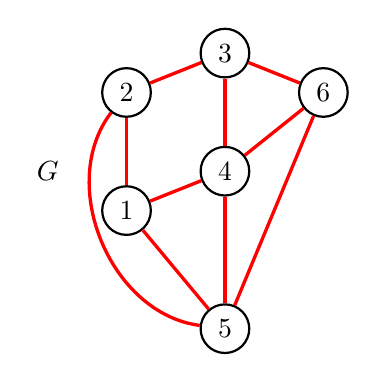
\begin{tikzpicture}[scale=0.5]
\begin{scope}[every node/.style={circle,thick,draw}]
    \node (A) at (0,0) {1};
    \node (B) at (0,3) {2};
    \node (C) at (2.5,4) {3};
    \node (D) at (2.5,1) {4};
    \node (E) at (2.5,-3) {5};
    \node (F) at (5,3) {6} ;
\end{scope}

\begin{scope}[>={Stealth[black]},
              every node/.style={fill=white,circle},
              every edge/.style={draw=red,very thick}]
    \path [-] (A) edge (B);
    \path [-] (B) edge   (C);
    \path [-] (A) edge   (D);
    \path [-] (D) edge   (C);
    \path [-] (A) edge   (E);
    \path [-] (D) edge   (E);
    \path [-] (D) edge  (F);
    \path [-] (C) edge  (F);
    \path [-] (E) edge   (F); 
    \path [-] (B) edge[bend right=60]  (E); 
    \end{scope} 
    \node at (-2,1) {$G$};    
  \end{tikzpicture}
  \qquad\qquad
  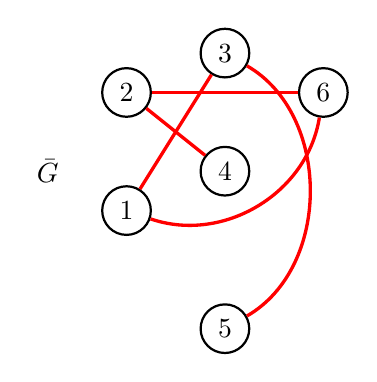
\begin{tikzpicture}[scale=0.5]
\begin{scope}[every node/.style={circle,thick,draw}]
    \node (A) at (0,0) {1};
    \node (B) at (0,3) {2};
    \node (C) at (2.5,4) {3};
    \node (D) at (2.5,1) {4};
    \node (E) at (2.5,-3) {5};
    \node (F) at (5,3) {6} ;
\end{scope}

\begin{scope}[>={Stealth[black]},
              every node/.style={fill=white,circle},
              every edge/.style={draw=red,very thick}]
    \path [-] (A) edge (C);
     \path [-] (A) edge [bend right=50] (F);
     \path [-] (B) edge (D);
     \path [-] (B) edge (F);
     \path [-] (C) edge[bend left=60] (E);
    \end{scope} 
\node at (-2,1) {$\bar{G}$};        
  \end{tikzpicture}
\caption{An example of an undirected graph $G$ with 6 vertices and 10 edges and its complment $\bar{G}$.}  
 \label{fig:graphs}
 \end{figure}
\end{center}
Such a graph  contains 6 vertices and 10 edges, its adiancency matrix is given by
\begin{equation}
 A=\begin{pmatrix}
    0& 1 & 0 & 1 & 1 & 0 \\
      1&  0 &  1& 0 & 1 & 0 \\
       0&1 & 0&1 & 0 & 1 \\
        1& 0 & 1 &  0& 1& 1 \\
        1 &1 &0 &1 & 0& 1 \\
         0& 0 & 1 & 1 & 1 & 0\\
   \end{pmatrix}.
\end{equation}
The graph $G$ is irregular, since in general different nodes have different degrees:
 $d_4=d_5=4$ and $d_1=d_2=d_3=d_6=3$.\\ 

\vspace{3mm}
\noindent
{\bf Spectral problem for the adiacency matrix.}
The adiacency matrix of an undirected graph $G$ is a simmetric non-negative $n\times n$ matrix
and its spectral problem is a classical problem in graph theory. Let us start considering the case of a regular
graph $G$ of degree $k$. For semplicity we will also assume the graph to be connected,
meaning that there is always a path connecting two arbirary vertices:
the adicency matrix $A$ is in this case irreducible and Perron-Frobenius theorem can be applied. 

It easy to show that the $n$-dimensional vector $|f\rangle$, with all entries equal 1
\begin{equation}
| f \rangle \,=\, \left(
\begin{array}{c} 
1 \\
1 \\
..\\ 
\\
..\\
\\
.. \\
1\\
1
\end{array}
\right)
\end{equation}
is an eigenvector of the adiacency matrix $A$ with eigenvalue $k$. Being its components all positive, $|f\rangle$ is actually 
the (unique) Perron Frobenius eigenvector of $A$ and therefore $k$ is also the largest eigenvalue of the matrix $A$. 
Moreover the one-dimensional eigenspace generated by $|f\rangle$ is orthogonal to all others eigenspaces of 
$A$ (being symmetric) and this implies that if $|v\rangle$ is an eigevector of $A$ with eigenvalue $\theta<k$ and we also have
\begin{equation}
\label{duality}
\bar{A}|v\rangle=(J-I-A)|v\rangle=(-1-\theta)|v\rangle.
\end{equation}
Note that analogously 
\begin{equation}
\bar{A}|f\rangle=(n-1-k)|f\rangle \,\,\,.
\end{equation}
If the $n$ real numbers $k>\theta_1\geq\theta_2\geq\dots\geq \theta_{n-1}$ are the spectrum of $A$, then we proved that the eigenvalues of $\bar{A}$ are $n-k-1>-1-\theta_{n-1}\geq -1-\theta_{n-1}\geq\dots\geq -1-\theta_1$. This observation furnishes an equation satisfied by the characteristic 
polynomials $P_{G}(x)$ and $P_{\bar{G}}(x)$  of the adiacency matrices of $G$ and $\bar{G}$. The characteristic polynomial of $G$ is indeed
\begin{equation}
P_{G}(x)\, =\, (x-k)\prod_{i=1}^{n-1}(x-\theta_i)\,\,\,,
\end{equation}
and one obtains 
\begin{equation}
\label{car_pol_reg}
 P_{\bar{G}}(x)=(-1)^{n}\frac{x-n+k+1}{x+k+1}P_{G}(-1-x)\,\,\,.
\end{equation}
The graph, whose adiacency matrix $A$ is the coprime matrix, is however irregular and the simple analysis outlined above for the spectral problem cannot be carried out. Here we simply quote the analogous results known for the largest eigenvalue $\lambda_{max}$ of the adiacency matrix and the characteristic polynomial of the  complementary graph. 

For irregular connected graphs the largest eigenvalue $\lambda_{max}$ of $A$ (that is unique and positive by the Perron Frobenius theorem) is bounded by the average degree $\bar{d}$ of the graph and its maximum degree $d_{max}$
\begin{equation}
 \bar{d}\leq\lambda_{max}\leq d_{max}\,\,\,.
\end{equation}
For a regular graph $G$ of degree $k$, $\bar{d}=d_{max}=k$ as we have already discussed. It is possible to generalize \eqref{car_pol_reg} to irregular graphs. Firstly we observe that $|f\rangle$ is no more an eigenstate of $A$ but nevertheless we can define the so-called \textit{main spectrum} of the graph $G$ as the vector space $M$ generated by all the eigenvectors of $A$ that are not orthogonal to $|f\rangle$. The main spectrum of a regular graph would be
one-dimensional and coinciding with the eigenspace of $|f\rangle$. 

With $|v_1\rangle,\dots,|v_{m}\rangle$ be the vectors of an ortonormalized basis for the main spectrum $M$, namely $A|v_i\rangle=\mu_i|v_i\rangle$ and $\langle v_i|f\rangle\not=0$, it is customary to introduce the angles $\beta_i$ of an irregular graph as $\beta_i=\frac{1}{\sqrt{n}}\langle f|v_i\rangle$, $i=1,\dots,m$.
Starting from the definition of the caracteristic polynomial of the complementary graph $\bar{G}$, $P_{\bar{G}}(x)=\det(\bar{A}-xI)$ and using the spectral decomposition of $A$, together with definition of $\bar{A}$, it is then possible to show that
\begin{equation}
\label{car_pol_irreg}
 P_{\bar{G}}(x)=(-1)^{n}P_{G}(-1-x)\left(1-n\sum_{i=1}^{m}\frac{\beta_i^2}{x+1+\mu_i}\right)\,\,\,,
\end{equation}
an equation that generalizes \eqref{car_pol_reg}.


\section{Maximum degree of the coprime graph in the limit $q \rightarrow \infty$}\label{Appmaxdegree}

\vspace{1mm}
\noindent
It is possible to estimate the rate of growth of the maximum degree of the coprime graph with the number $q$  based using as hypothesis the statistical independence of the primes. The argument goes as follows. Given a number $q$, firstly let's determine which is the maximum index $s$ such that the 
number made of the product of the first $s$ consecutive primes is less than $q$ 
\be 
\hat n \,=\, p_1 \times p_2 \ldots \times p_s \,< \, q \,\,\,.
\label{goodnumber}
\ee
Such number $\hat n$ is associated to one of the vertices with the maximum degree in the range $(2,q)$. In fact, this number divides all numbers multiples of $p_1 =2$, all those which are multiples of $p_2 = 3$, all those multiples of $p_3 = 5$, etc. Let's now estimate how many numbers have common factors with 
$\hat n$ using a probability argument. 

The total number of numbers that are divisible by $2$ is given by $q$ times the probability that a number is divisible by $2$, which is $\frac{1}{2}$, so $q \times \frac{1}{2}$. The total number of those which are divisible by $3$ are given, naively, by $q \times \frac{1}{3}$. However this is an over-counting since among these multiples of $3$ there are those we have already counted as divisible by $2$ (as, for instance, the number $6$) and therefore we have to subtract them. So the genuine numbers which are divisible by $3$ but not also by $2$ are given by $q$ multiplied for the probability $\hat p_3$ that a number is divisible by $3$ but not by $2$ 
\be 
\hat p_3 \,=\,\frac{1}{3} \, \left(1 - \frac{1}{2}\right) \,\,\,. 
\ee
Analogously, we can count the genuine numbers divisible by $5$ but not divisible for $2$ and $3$, in term of the corresponding probability 
\be 
\hat p_5 \,=\,\frac{1}{5} \,\left(1 - \frac{1}{2}\right) \, \left(1 - \frac{1}{3}\right) 
\ee 
and, more generally, 
\be 
\hat p_k \,=\,\frac{1}{p_k} \,\prod_{m=1}^{k-1} \left(1 - \frac{1}{p_m}\right) \,\,\,.
\ee
In this way, we predict that the maximum degree grows as 
\be 
d_{max} \,\sim\, q \, \sum_{k=1}^s \hat p_k \,\,\,.
\label{estmd}
\ee 
Notice that the number of terms included in the sum depends on the number $q$ itself: therefore there will be a sequence of discontinuities of the 
corresponding slope each time that $q$ overpass the values 
\be
2\, ,6 \,, 30\,, 210 \,, 2310 \,, 30030 \, \ldots 
\ee 
associated to the sequence of numbers $\hat n$. This explains why the slope of the maximum degree changes by changing the the upper value $q$ 
giving rise to a pronounced finite-size dependence as commented in the text.  

However, in the asymptotic limit $q\rightarrow \infty$, we have that also the maximum index $s$ goes to infinity, $s \rightarrow \infty$, and therefore the 
ratio $d_\mathrm{max}/q$ is given by the infinite series 
\be \label{pseries}
\frac{d_\mathrm{max}}{q} \underset{ q \to \infty }{ \sim } \sum_{n=1}^\infty \,\frac{1}{p_n} \prod_{m=1}^{n-1} \left(1 - \frac{1}{p_m}\right)
\ee
The series is convergent since
\be \label{hseries}
\sum_{n=1}^\infty \,\frac{1}{p_n}  \exp \( \sum_{m=1}^{n-1} \left(1 - \frac{1}{p_m} \right) \) < \sum_{n=1}^\infty \,\frac{1}{p_n}  \exp \( - \sum_{m=1}^{n-1}  \frac{1}{p_m}  \) < \sum_{n=1}^\infty \,\frac{1}{p_n}  \frac{ e^{ \frac{\pi^2}{6} }}{ \log {p_n}  }\,\,\,,
\ee 
where the last inequality follows from the fact that the truncated sum of the reciprocals of the primes is bounded by
\be 
\sum_{p < n } \frac{1}{p} > \log \log n - \log \frac{\pi^2}{ 6 } \,\,\,.
\ee
The series in the last member of \eqref{hseries} converges as a consequence of the prime number theorem, which states that the magnitude of the $n$-th prime number goes as
\be 
p_n \underset{ n \to \infty }{ \sim }  n \log n\,\,\,,
\ee
so that the general term behaves asymptotically as
\be 
\frac{1}{ p_n \log p_n } \underset{ n \to \infty }{ \sim } \frac{1}{ n (\log n)^2 }
\ee
which is enough to make the series convergent.

Since the maximum degree of a graph cannot exceed the number of vertices of the graph, the series \eqref{pseries} must converge to a value smaller or equal to $1$. As a matter of fact the result is exactly $1$, as the truncation of the series \eqref{pseries} can be put in the telescopic form
\begin{align*}
\sum_{n=1}^N \, \(1 - 1 + \frac{1}{p_n} \) \prod_{m=1}^{n-1} \left(1 - \frac{1}{p_m}\right)  & = 
\sum_{n=1}^N {} \prod_{m=1}^{n-1} \left(1 - \frac{1}{p_m}\right) - \sum_{n=2}^{N+1} {} \prod_{m=1}^{n-1} \left(1 - \frac{1}{p_m}\right)  =  \\[1mm]
& =  1 - \prod_{m=1}^{N} \left(1 - \frac{1}{p_m}\right)  \quad \underset{ N \to \infty }{  \rightarrow } \quad  1  - \frac{1}{ \zeta(1) } = 1 
\end{align*}
where
\be 
\zeta(z) = \prod_{k=0}^{\infty} \(1 - p_k^{-z} \)^{-1}
\ee
is the product representation of the Riemann Zeta function, whose only pole is $z=1$.

In summary, for asymptotically large values of $q$ the maximum degree of the coprime graph scales exactly as $q$ 
\begin{equation}
d_m \simeq q 
\,\,\,\,\,\,\,\,\,
,
\,\,\,\,\,\,\,\,\,
q \rightarrow \infty
\end{equation}

\section{Eigenvalues of the coprime matrix in the limit $q \rightarrow \infty$}
\centerline{Appendix written by Don Zagier}


\newpage

\begin{thebibliography}{1}
\bibitem{Rimenboim1} P. Rimenboim, {\em The little book of bigger prime numbers}, 2004 Springer-Verlag New York, Inc. 
\bibitem{Rimenboim2} P. Rimenboim, {\em My Numbers, My Friends: Popular Lectures on Number Theory}, 2000 Springer-Verlag New York, Inc.
\bibitem{Schroeder} M. R. Schroeder, {\em Number Theory in Science and Communications}, 1990 Springer-Verlag New York, Inc.
\bibitem{Zagier} D, Zagier, {\em The first 50 Million Prime Numbers}, The Mathematical Intelligencer, Vol. 0,. August 1977.
\bibitem{Young} R.M. Young, {\em Excursions in Calculus. An Interplay of the Continuous and the Discrete}, Dolciani Mathematical Expositions Number 13, The Mathematical Association of America 1992.  
\bibitem{Riemann} B. Riemann, {\em Ueber die Anzahl der Primzahlen unter einer gegebenen Gr�sse}, Monatsberichte der Berliner Akademie, 
In Gesammelte Werke, Teubner, Leipzig (1892). 
\bibitem{Hardy} G. H. Hardy and  E.M. Wright, {\em An Introduction to the theory of numbers}, Oxford University Press, Oxford 1938. 
\bibitem{Baker} A. Baker, {\em A concise introduction to the theory of numbers}, Cambridge University Press, Cambridge 1984. 
\bibitem{Apostol} T.M. Apostol, {\em Introduction to analytic number theory}, Undergraduate Texts in Mathematics, New York-Heidelberg: Springer-Verlag, 1976. 
\bibitem{Manin} Yu. I. Manin and A.A. Panchishkin, {\em Introduction to Modern Number Theory}, Springer Berlin Heidelberg New York 2005. 
\bibitem{Edwards} H. M. Edwards  {\em Riemann's Zeta Function},  Academic Press 1974. 
\bibitem{Tichmaesh} E.C. Titchmarsh, {\em The Theory of the Riemann Zeta Function}, Oxford University Press 1986. 
\bibitem{Conrey} J. B. Conrey, The Riemann Hypothesis, Notices of the AMS 50 (2003) 342.
\bibitem{Bombieri} E. Bombieri, Problems of the Millennium: The Riemann hypothesis, Clay Mathematics Insti-
tute (2000).
\bibitem{Sarnak} P. Sarnak, Problems of the Millennium: The Riemann hypothesis, Clay Mathematics Institute
(2004).
\bibitem{Mazur} B. Mazur and W. Stein, {\em Prime Numbers and the Riemann Hypothesis}, Cambridge University Press, Cambridge 2016.
\bibitem{Polya} G. Polya, unpublished (c. 1914). See A. Odlyzko, Correspondence about the origins of the Hilbert - Polya conjecture,
http://www.dtc.umn.edu/?odlyzko/polya/index.html (1981-1982).
\bibitem{Berry} M.V. Berry, {\em Riemann�s zeta function: a model for quantum chaos?}, Quantum Chaos and Statistical Nuclear Physics, 
ed. T. H. Seligman and H. Nishioka vol 263, 1-17, 1986; M.V. Berry, Nonlinearity 1 399-407 (1988); 
M. V. Berry and J. Keating, SIAM Review 41, 236 (1999). 
\bibitem{Connes} A. Connes,  Sel. Math., New Ser. 5, 29 (1999) [arXiv:math/9811068]. 
\bibitem{Sierra} G. Sierra, Nucl. Phys. B 776, 327 (2007) [arXiv:math-ph/0702034]; G. Sierra, J. Stat. Mech. 0512, P006 (2005) [arXiv:math.nt/0510572]; 
G. Sierra, New J. Phys. 10, 033016 (2008) [arXiv:0712.0705 [math-ph]]; G.Sierra, P.K. Townsend, Phys.Rev.Lett.101, 110201 (2008) [arXiv:0805.4079 [math-ph]]; 
G. Sierra, {\em The Riemann zeros as spectrum and the Riemann hypothesis} [ArXiv: 1601.01797 [math-ph]]. 
\bibitem{Leclair} G. Fran�a, A. LeClair, Communications in Number Theory and Physics, Vol. 9, No. 1 (2015); A. LeClair, Int. J. Mod. Phys. A28 (2013) 1350151. 
\bibitem{Schumayer} D. Schumayer and D. A. W. Hutchinson, Rev. Mod. Phys. 83 (2011) 307 [arXiv:1101.3116].
\bibitem{GMussardo} G. Mussardo, {\em The Quantum Mechanical Potential for the Prime Numbers}, arXiv:cond-mat/9712010. 
%\bibitem{Montgomery} H.L. Montgomery, Analytic number theory, Proc. Symp. Pure Math. 24,181 (1973). 
%\bibitem{Mehta} M. L. Mehta, Random Matrices, Elsevier Ltd. The Netherlands, 2004.
\bibitem{ent1} C. Holzhey, F. Larsen and F. Wilczek, Nucl. Phys. B  424, 443, (1994) 
\bibitem{ent2} G. Vidal, J.I. Latorre, E. Rico, and A. Kitaev, Phys. Rev.  Lett. 90 ,227902-1 (2003) 
\bibitem{ent3} V.E. Korepin, Physical Review Letters, vol 92,  096402, 2004. 
\bibitem{ccee} J. L. Cardy, P. Calabrese, \emph{Entanglement Entropy and Quantum Field Theory}, J. Stat. Mech. (2004). 
\bibitem{Schroeder2} M.R.Schroeder, Mathematical Intellingencer 4, 158-161 (1982). 
\bibitem{kogut} J. B. Kogut, \emph{An introduction to lattice gauge theory and spin systems}, Rev. Mod. Phys. 51, 659 (1979).
\bibitem{metro} N. Metropolis, A. W. Rosenbluth, M. N. Rosenbluth, A. H. Teller, E. Teller, \emph{Equations of State Calculations by Fast Computing Machines}, J. Chem. Phys. 21 (6), 1087–1092 (1953).
\end{thebibliography}

\end{document}

